\chapter{Maternal Methylmercury Exposure through Rice Ingestion during Pregnancy}

\section{Introduction}

Methylmercury (MeHg) is one of the most toxic forms of mercury (Hg); it has been implicated as a neurotoxin in biologic organisms \citep{clarkson2006toxicology}. Human MeHg exposure has been a public health problem for many decades (World Health Organization, 1990). For the general population, the primary pathway of MeHg exposure is dietary exposure via consuming fish/shellfish or sea mammals \citep{mergler2007methylmercury}. MeHg can cross the placenta and pass through the blood-brain barrier; the developing fetus is considered to be more vulnerable to the adverse effects of MeHg exposure than adults (National Research Council, 2000).

Recently, rice consumption has received attention as a potential MeHg exposure pathway. Rice is grown in rice paddy fields (stagnant water), which are favorable sites for the methylation of Hg: inorganic Hg (\(\text{Hg}^{2+}\)) is converted to MeHg by anaerobic microbes \citep{rothenberg2014rice}. Then MeHg is likely translocated from rice paddy soil to rice grain \citep{rothenberg2014rice}. Additionally, rice is widely cultivated around the world and is a staple food for more than half of the world's population \citep{mohanty2013trends}. In some areas where rice is a staple food and Hg contamination is elevated, rice consumption has been reported as being an important human MeHg exposure pathway \citep{feng2007human,liang2015human}. 

Some epidemiological studies have reported data for rice ingestion or rice Hg intake, rice total Hg (THg) or MeHg concentrations, and human Hg exposure, measured in hair, blood, or urine (Table 2.1). A few of the studies summarized in Table 2.1 observed positive correlations between Hg biomarkers and rice consumption, rice MeHg intake, or rice MeHg concentrations. For example, four studies conducted in a Hg mining area of Guizhou Province, China all found similar results. First, \cite{feng2007human} reported that the rice MeHg intake positively correlated with hair MeHg levels (r=0.65, p<0.01, n=98) and indicated that the rice MeHg intake contributed > 90\% of the total dietary MeHg intake (food sources: rice, meat, vegetables, and drinking water) in the study populations. Second, \cite{li2011human} reported that the rice MeHg intake positively correlated with hair MeHg levels (r=0.73, p<0.001, n=43). Third, \cite{li2015humanbb} observed significantly positive correlations between the rice MeHg intake and MeHg concentrations in hair or blood (\(\text{r}^{2}\) =0.74-0.83, p<0.001, n=168). Lastly, \cite{rothenberg2013prenatal} reported that rice MeHg concentrations were positively correlated with maternal hair THg and MeHg and blood THg in a cohort of pregnant women (\(\text{r}^{2}\) =0.31-0.66, n=17). Moreover, a U.S. study [National Health and Nutrition Examination Survey, (NHANES)] found that rice consumption was positively correlated with blood THg in both children and adults in unadjusted analyses (n=16236), and observed that an increase of 10 g/day of rice consumption was associated with a 4.8\% increase in blood THg concentration in adjusted models for adults (n=10373) \citep{davis2014dietary}. However, a Korean study (n=3404) reported that the blood Hg levels were not associated with rice consumption in the logistic models adjusted for sex, age, residence area, education, body mass index (BMI) and smoking and drinking status \citep{park2013strong}. 

Rice does not contain the same beneficial nutrients as fish/shellfish, such as n-3 polyunsaturated fatty acids \citep{rothenberg2011low}. Maternal MeHg exposure mainly through rice ingestion may increase adverse effects in the developing fetus without the nutritional benefits from the consumption of fish/shellfish. Yet, to our knowledge, only two studies \citep{maramba2006environmental, rothenberg2013prenatal} reporting rice Hg concentrations or rice ingestion and Hg biomarker levels were conducted in pregnant cohorts. Both of them were conducted in Hg contaminated regions and had a small sample size (n=35, \cite{maramba2006environmental}; n=17, \cite{rothenberg2013prenatal}).

China is the largest rice producer in the world, accounting for 27.6\% of the world's rice production \citep{fao2016}. Just like a Chinese proverb says, ``A meal without rice just isn't a meal''. In most regions of Asian countries, rice is so central to the culture that the word ``rice'' is almost synonymous with food. However, there are very few studies about human MeHg exposure through rice ingestion among pregnant women. Thus this study was pursued to investigate the magnitude of MeHg exposure among pregnant women in an inland area of China where rice is a staple food, and to determine the importance of rice and fish/shellfish as sources of dietary MeHg intake.

\section{Methods}

\subsection{Study site and recruitment}

This study was conducted in Daxin County, Guangxi Zhuang Autonomous Region, China (Figure 2.1). Daxin is situated in the inland of southern China, near the China-Vietnam border, where the total land area is 2,742 \(\text{km}^{2}\) and the population was 359,800, including \({\sim}\)50,000 (14\%) living in the town of Daxin. Daxin is an agriculture-oriented county; the main crops are rice, corn, sugarcane, and soybean \citep{daxin2016} . There were no significant sources of Hg nearby, such as coal-fired power plants.

Between May 2013 and March 2014, pregnant women were recruited at parturition at the Maternal and Child Health Hospital in Daxin County. Eligibility criteria were that the participants were in good health generally, had resided in Daxin County during the three previous months, planned to remain living in Daxin for the next year, and were currently not under treatment for a chronic disease. 

This study was approved by the Institutional Review Boards at the University of South Carolina (USA) and Xin Hua Hospital (China). The mothers also provided written informed consent before the enrollment. 

\subsection{Samples collection}

Upon enrollment, trained nurses collected a maternal hair sample from the occipital region using stainless scissors. The proximal end was tied with dental floss, and the hair samples were individually stored in plastic bags at room temperature. A maternal blood sample was collected by venipuncture (6 ml) into two vials, including one with lithium heparin anticoagulant, and the second vial for separation of serum by centrifugation (3600 rpm, 10 min) \citep{yu2011prenatal}. Whole blood and an aliquot of serum were stored frozen at -26\({^\circ}\)C for up to 10 months, then stored at -80\({^\circ}\)C until analysis. A family member brought a \({\sim}\)100 g rice sample from home (all participants donated rice samples), which was stored frozen at -26\({^\circ}\)C, and then archived at -80\({^\circ}\)C until analysis. 

In May 2014, 13 freshwater tissue samples (including seven species commonly consumed by residents: common carp = 2, tilapia = 2, silver carp = 2, catfish = 2, grass carp = 2, bighead carp = 2, and mud carp = 1) were collected from two local markets in Daxin. Fresh freshwater fish tissue was individually stored in plastic bags and immediately stored frozen at - 26\({^\circ}\)C, then samples were transported frozen to Lumex's lab in Beijing using Credo Cube (Pelican BioThermal, Plymouth, MN USA), which can keep samples frozen at - 26\({^\circ}\)C for three days.

\subsection{Data collection}

While in the hospital, mothers filled out a questionnaire that included information such as maternal age at parturition (years), maternal height and weight before pregnancy, maternal ethnicity, maternal education, maternal occupation, monthly household income, smoking during pregnancy, secondhand smoke during pregnancy, and alcohol consumption during pregnancy. 

Additionally, mothers filled out a modified semi-quantitative food frequency questionnaire (FFQ) about their food consumption during the third trimester. This valid FFQ has been used for a study of dietary intake among pregnant women living in a rural area of western China \citep{cheng2009assessment}. The FFQ involved 102 items, including rice, fish/shellfish, and other foods. Mothers were asked to choose from eight options ranging from ``never or rarely'' to ``twice/day'', and these frequencies were converted to servings/day as follows: 0 = never or rarely, 1/30.5 = monthly, 2.5/30.5 = two to three times/month, 1/7 = once/week, 2.5/7 = two to three times/week, 5/7 = four to six times/week, 1= once/day, and 2.5 = at least twice/day. For rice consumption, mothers were also asked to select portion size (g/serving) from one of three bowls using a picture and/or actual bowls (85 g/bowl, 135 g/bowl, 260 g/bowl). The daily rice ingestion rate (g/day) was calculated by multiplying the consumption frequency (servings/day) \({\times}\) the portion size (g/serving). 

For fish/shellfish consumption, mothers reported the consumption frequency for seven categories of fish/shellfish (including freshwater fish, marine fish, eel, shrimp, crab, snails, and other shellfish) using the same eight options (from ``never to rarely'' to ``twice/day''), then these frequencies were converted to servings per day as described above for rice consumption. To calculate fish/shellfish ingestion rate (g/day), we assumed 170 g/serving for marine fish and freshwater fish (170 g = 6 ounces, the recommended serving size from the \citep{usfda2011fish}, and 100 g/serving for other categories (eel, shrimp, crab, snails, and other shellfish) \citep{cheng2009assessment}. 

\subsection{Dietary MeHg intake assessment}

Dietary MeHg intake through rice or fish/shellfish consumption (\({\mu}\)g/day) was quantified by multiplying the ingestion rate (g/day) \({\times}\) the average concentrations of rice MeHg (\({\mu}\)g/g) or fish/shellfish THg (\({\mu}\)g/g). Rice MeHg concentration was measured in each participant's donated rice sample. In this study, we measured rice MeHg (not THg) due to the rice MeHg\% (of THg) ranging from 17\% to 75\% \citep{rothenberg2014rice}, while fish MeHg\% (of THg) was greater than 90\% (National Research Council, 2000). For the THg concentrations of fish/shellfish, freshwater fish THg concentrations were measured in freshwater fish tissue samples collected from Daxin markets, while THg concentrations of other fish/shellfish varieties (including marine fish, eel, shrimp, crab, snails, and other shellfish) were obtained from a comprehensive literature search. 

The literature search was conducted using the Thomas Reuters (ISI) Web of Science and the phrase ``mercury and China'', which was combined with ``seafood'', ``fish'', ``eel'', ``shrimp'', ``crab'', ``mollusk'', ``shellfish'', ``snail'', ``scallop'', ``oyster'', ``lobster'', ``spiral shell'', or ``bivalve'', resulting in 209 studies. Studies were included if they were conducted in non-contaminated sites in China, THg (or MeHg) concentrations were reported in wet weight, and most or all fish/shellfish samples were collected after 1 January 2011. For ``eel'', just one study for China was published in 2006 and was included. Therefore, a total of 12 studies were finally included (Table 2.2 and Figure 2.2). Summary statistics [mean, standard deviation (SD), median, and range] were calculated for each fish/shellfish variety if possible. For studies reporting the sample size, mean, SD and median were calculated using the sample size as the analytical weight. 

Total dietary MeHg intake through rice and fish/shellfish consumption (\({\mu}\)g/day) was equivalent to the daily rice MeHg intake + the daily fish/shellfish MeHg intake. Proportional contributions from rice or fish/shellfish consumption were also determined. 

\subsection{Laboratory analyses}

\subsubsection{Labware preparation for Hg analyses}

Prior to Hg analyses, all lab wares were acid-washed for > 24 hours using 1.2 N hydrochloric acid, then triple-rinsed with deionized-water (DDI-H2O) (resistivity: > 18.0 M\({\Omega}\)/cm, Barnstead water system, Thermo Scientific, US), and dried in a biosafety Hood (Baker Company, Sanford, USA) to prevent further Hg contamination, then double-bagged for later use. 

\subsubsection{Maternal hair THg and MeHg and blood THg analyses}

Hair samples corresponding to the third trimester (34 mm) were analyzed, assuming a growth rate of 0.41 mm/day for Asian women \citep{loussouarn2005diversity}, and 83 days for the third trimester, reflecting a 10-day lag between Hg ingestion and incorporation of MeHg into the hair shaft \citep{cernichiari1994biological}. Prior to the hair THg and MeHg measurement, two hair washing methods were compared, including 1\% (v/v) Formula 409\textsuperscript{TM} and 0.1\% (v/v) 2-mercaptoethanol. Formula 409\textsuperscript{TM} is considered to be more effective than acetone (the International Atomic Energy Agency hair washing method) \citep{rothenberg2013prenatal}, while 2-mercaptoethanol can remove high concentrations of inorganic Hg from hair \citep{li2011human}, as well as plant material \citep{north2000heterogeneity}. Six random hair samples were weighted into 12 acid-washed 120 mL porcelain dishes, 25 mL of 1\% (v/v) Formula 409\textsuperscript{TM} or 0.1\% (v/v) 2-mercaptoethanol were each added into six dishes, respectively. Samples were gently shaken for 1 hour, 60-70 rpm (HS 501 Digital Orbital And Reciprocal Shakers, IKA Works, Inc., USA), then triple-rinsed with DDI-H2O, and air-dried in a biosafety Hood (Baker Company, Sanford, USA). The comparisons showed that 2-mercaptoethanol removed on average 19\% more exogenous Hg than Formula 409\textsuperscript{TM} did (Table 2.3). Therefore, 0.1\% (v/v) 2-mercaptoethanol was used for all hair samples. After the hair washing, hair samples were individually bagged and stored until analysis. Blood samples were analyzed directly, and no preparatory steps were needed.

THg concentrations for maternal hair and blood were measured by thermal decomposition, amalgamation and atomic absorption spectrophotometry following EPA Method 7473 \citep{usepa2007m7473} using a Lumex for hair (Model RA-915+/PYRO-915+, St. Petersburg, Russia), and a DMA-80 for blood (Milestone, Inc., Shelton, CT, USA).

For hair MeHg analysis, washed hair samples were weighted into 50 mL Teflon tubes (Savillex, MN, USA) and 5 mL of 25\% (w/v) sodium hydroxide-DDI H2O were added, and samples were digested for 3 hours at 75\({^\circ}\)C in an oven. Just before the measurement, boiling DDI-H2O was added to a total volume of 50 mL (personal communication, Lian Liang, CEBAM Analytical, Inc., Seattle, WA, US). Digests were analyzed following EPA Method 1630 \citep{usepa1630}, including ethylation with sodium tetraethylborate, purge and trap onto Tenax traps, and quantification using gas chromatography-cold vapor atomic fluorescence spectrometry (GC-CVAFS, Brooks Rand Model III, Seattle, WA, USA). 

\subsubsection{Rice MeHg analysis}

Rice samples were grounded into a powder using a coffee grinder (Cool Grind Coffee Grinder, Model \# 501, Capresso), which was cleaned with ethanol after each sample to prevent carry-over of Hg. Rice MeHg was extracted following \cite{liang1996simple}. \({\sim}\) 0.5 g rice was weighted into 50 ml Falcon tubes (Fisher Scientific, PA, USA), then 2 mL of 25\% (w/v) potassium hydroxide - methanol were added for digestion, heating for 3 hours at 75\({^\circ}\)C. After cooling down to room temperature, 6 mL of dichloromethane and 1.5 mL hydrochloric acid were added, then samples were shaken for 30 min, centrifuged  (4000 rpm, 20\({^\circ}\)C) for 30 min, and the phases were separated, the phase of extracts were collected into 50ml Falcon tubes (Fisher Scientific, PA, USA). DDI-H2O was added, and samples were heated for 1.5 hours in a water bath at 60-75\({^\circ}\)C to expel dichloromethane. Extracts were measured using the EPA Method 1630 as described above for MeHg \citep{usepa1630}.

\subsubsection{Freshwater fish THg analyses}

Freshwater fish THg were measured directly following the EPA Method 7473 (U.S. Environmental Protection Agency, 2007) and using a Lumex (Model RA-915+/PYRO-915+, St. Petersburg, Russia) as described above for the hair THg. The THg concentrations of freshwater fish were reported as wet weight. 

\subsubsection{Quality assurance/quality control (QA/QC) for Hg analyses}

QA/QC for Hg analyses were summarized in Table 2.4. For hair, rice and fish tissue, the average recovery of standard reference material ranged from 78\% to 96\%, matrix spikes averaged 96-98\%, and the average relative percent difference between samples replicates ranged from 4.2\% to 8.4\%. For blood THg, recovery of standard reference material ranged from 85\% to 110\%, and the relative percent difference between sample replicates was < 20\%. The limits of detection were instrument-specific and matrix-specific, including hair THg (0.0095 \({\mu}\)g/g), hair MeHg (0.0001 \({\mu}\)g/g), blood THg (0.14 \({\mu}\)g/L), fish THg (0.001 \({\mu}\)g/g), and rice MeHg (0.002 ng/g). All observations were above the limits of detection.

Rice and hair THg and/or MeHg analyses were completed at the University of South Carolina, USA, fish tissue THg was analyzed at Beijing Lumex Analytical Co. Ltd., China, and blood THg was analyzed at the Shanghai State Key Lab for Children's Environmental Health, China.

\subsubsection{Statistics}

Data were assessed using univariate and bivariate analyses. Correlations were determined using Spearman's correlation (for non-symmetrical variables) or Pearson's correlation (for symmetrical variables). For Pearson's correlation, a $\log_{10}$-transformation was applied to variables with a right-skewed distribution. Prior to the $\log_{10}$-transformation, a value of 0.01 was added to all observations for fish/shellfish MeHg intake (\({\mu}\)g/day), because more than 40\% of the mothers reported that they rarely or never ingested fish/shellfish. 

For the rice consumption responses, 5.5\% of mothers did not choose a frequency (servings/day) or quantity (g/serving). Missing observations were imputed based on the multivariate normal distribution \citep{schafer1997analysis}, conditional on biomarker concentrations and maternal, paternal and offspring characteristics. For the fish/shellfish consumption responses, 4.3\% of the participants did not choose a frequency for one or more fish/shellfish categories, and a value of 0 was imputed for these observations, which was appropriate for this inland region in rural China. We assumed participants skipped some categories for fish/shellfish because these varieties were often unavailable in Daxin. 

We defined an alpha-level < 0.05 as a guide for significance. Analyses were performed using SAS 9.4 software (SAS Institute Inc., Cary, NC, USA) or the R-platform.

\section{Results}

\subsubsection{Characteristics of the participants}

During the recruitment period, 1261 women visited the Maternal and Child Health Hospital of Daxin County. Among these women, 408 (32\%) were eligible for the study and provided informed consent, while 853 were ineligible due to infectious disease (e.g., Hepatitis B) (n=228), residence outside Daxin (n=574), or refused to participate (n=51). Ten mothers were subsequently excluded because they did not give birth in the hospital (n=1), gave birth to twins (n=1), did not live in Daxin during the previous three months (n=3), or did not complete the data collection (n=5). Finally, 398 pregnant women were recruited. 

The average maternal age at parturition was 28 \({\pm}\) 5.7 years. For the pre-pregnancy BMI, 59\% of the mothers had normal BMI (BMI < 18.5 kg/\(\text{m}^{2}\)), 24\% were classified as underweight (18.5 kg/\(\text{m}^{2}\) ${\le}$ BMI < 23 kg/\(\text{m}^{2}\)), and 17.3\% were classified as overweight (23 kg/\(\text{m}^{2}\) ${\le}$  BMI < 27.5 kg/\(\text{m}^{2}\)) or obese (BMI ${\ge}$ 27.5 kg/\(\text{m}^{2}\)) \citep{who2004appropriate}. A majority of mothers were ethnic minorities (including 85\% Zhuang and 2\% other ethnic groups), and 13\% were Han (the largest ethnic group in China). Additionally, 93\% of the participants had an education level of high school or below, and only 5\% had a university degree. 76\% of these mothers were farmers, while 8.0\% were workers (including civil servants, white-collar workers, skilled/unskilled workers, or shopkeepers), 11\% were unemployed, and 3.3\% selected ``other'' for occupations. 59\% of the participating families had a monthly household income below 2000 renminbi (RMB), and 5.0\% had a household income above 5000 RMB. Among mothers in our cohort, 54\% were exposed to secondhand smoke, while very few mothers smoked during pregnancy (1.3\%), suggesting higher smoking among males compared to females. Differences in smoking observed in this cohort are similar to other Chinese populations (e.g. 56.75\% male vs. 6.7\% female in 27 cities, \cite{yang2015impact}). Lastly, just 1.0\% of the mothers reported consuming alcohol during pregnancy. Distributions of these maternal characteristics are shown in Figures 2.3 and 2.4.

\subsubsection{Rice and fish/shellfish Hg concentrations}

In the Daxin cohort, the geometric mean rice MeHg levels (2.1 ng/g) was close to 2.5 ng/g (the average rice MeHg concentrations for non-polluted sites reported from \cite{rothenberg2014rice}), and 92\% (n=367) of rice MeHg concentrations were less than 5.8 ng/g (the maximum rice MeHg concentrations for non-polluted sites reported from \cite{rothenberg2014rice}) (Table 2.5 and Figure 2.5).

The THg concentrations for freshwater fish purchased in Daxin markets averaged 31 \({\pm}\) 31 ng/g (n = 13). This THg concentration was 16 times lower than the Chinese dietary guideline (500 ng/g from \cite{usda2014china}), and ten times lower than the US EPA human health criterion (300 ng/g from \cite{usepa2001water}). Additionally, the average THg concentrations for fish/shellfish (range: 10 - 56 ng/g) obtained through a literature search were also up to 30 times lower than the US EPA criterion \citep{usepa2001water} (Table 2.5 and Figure 2.5). 

\subsubsection{Food ingestion and dietary MeHg intake}

In the Daxin cohort, 82\% of the mothers (n=328) reported consuming rice daily, and only three mothers reported rarely or never ingesting rice. On average, mothers consumed 1.8 servings/day of rice (median: 2.5 servings/day, range: 0-2.5 servings/day). The estimated rice ingestion rate averaged 231 \({\pm}\) 120 g/day (median: 213 g/day, range: 0-650 g/day), which was similar to the rate of the general Chinese population (Food and Agriculture Organization of the United Nations, 2016). While for the fish/shellfish consumption, almost half of the mothers (43\%) reported that they rarely or never consumed fish/shellfish, 180 mothers (45\%) reported consuming fish/shellfish < twice/week, and 45 mothers (11\%) reported consuming fish/shellfish ${\ge}$ twice/week. The fish/shellfish ingestion frequency averaged 0.13 servings/day (median: 0.03 servings/day, range: 0-2.9 servings/day), which was 14 times lower than the rice consumption frequency (1.8 servings/day). Additionally, on average mothers ingested 18 \({\pm}\) 45 g/day of fish/shellfish (median: 5.6 g/day, range: 0-470 g/day), which was lower than the average rate in China (95 g/day, from Food and Agriculture Organization of the United Nations, 2016). 

The estimated daily MeHg intake through rice and fish/shellfish ingestion was calculated using mothers' responses recorded in the FFQ and the MeHg concentrations of rice and THg concentrations of fish/shellfish. On average, mothers ingested 0.63 \({\pm}\) 0.65 \({\mu}\)g/day MeHg through rice ingestion (median: 0.44 \({\mu}\)g/day, range: 0-5.0 \({\mu}\)g/day) and 0.60 \({\pm}\) 1.6 \({\mu}\)g/day MeHg through fish/shellfish ingestion (median: 0.15 \({\mu}\)g/day, range: 0-8 \({\mu}\)g/day). The estimated total MeHg intake from rice and fish/shellfish averaged 1.2 \({\pm}\) 1.8 \({\mu}\)g/day (median: 0.77 \({\mu}\)g/day, range: 0-20 \({\mu}\)g/day), including 71 \({\pm}\) 33\% from rice consumption (median: 87\%, range: 0-100\%) and 29 \({\pm}\) 33\% from fish/shellfish consumption (median: 13\%, range: 0-100\%). Our findings indicated that maternal rice ingestion was a significant dietary MeHg exposure pathway in this cohort.  Detailed results are summarized in Table 2.6 and Figures 2.6 and 2.7.

\subsubsection{Hg biomarkers}

THg and/or MeHg concentrations in maternal hair and blood are summarized in Table 2.6 and Figure 2.8. 12 mothers (3.0\%) had hair THg concentrations greater than 1.1 \({\mu}\)g/g, corresponding to the US EPA recommended hair THg level \citep{usepa1997hgcongress}. Four pregnant women (1.00\%) had blood THg levels exceeding 5.8 \({\mu}\)g/L, which is the level suggested by the National Research Council (2000). Only one mother had Hg biomarker concentrations exceeding both the National Research Council recommended levels for blood and the US EPA recommended levels for hair.

Hair THg and MeHg concentrations were highly correlated (Spearman's rho = 0.92, p < 0.001, n = 398), and both were positively correlated with blood THg concentrations (for both: Spearman'ss rho = 0.69, p < 0.001). After $\log_{10}$-transformation, $\log_{10}$ hair THg and $\log_{10}$ MeHg were still strongly correlated (Pearson's rho=0.92, p < 0.001, n=398), and both were positively correlated with $\log_{10}$ blood THg (for both, Pearson's rho = 0.67-0.69, p < 0.001) (Figure 2.9). 

\subsubsection{Bivariate analyses}

\paragraph {Dietary MeHg intake through rice or fish/shellfish ingestion and Hg biomarkers}: \\ We found weakly positive and significant relationships between all Hg biomarkers and rice MeHg intake (\({\mu}\)g/day) in this cohort (Spearman's rho=0.17-0.21, p<0.001 for all biomarkers) (Figure 2.10). Trends were similar after applying the $\log_{10}$-transformation (Pearson's rho=0.20-0.22, p<0.001 for all biomarkers) (Figure 2.10). When using the rice consumption frequency (servings/day), the trends were still positive, but only significant for hair THg and blood THg (Spearman's rho: 0.10-0.11, p < 0.05 for both biomarkers) and non-significant for hair MeHg (Spearman's rho=0.07, p=0.18) (Figure 2.11). 

In contrast, we observed non-significant correlations between all Hg biomarkers and the fish/shellfish consumption frequency (servings/day) (Spearman's rho: 0.03-0.08, p=0.14-0.54 for all biomarkers) (Figure 2.12), and the fish/shellfish MeHg intake (\({\mu}\)g/day) (Spearman's rho=0.04-0.08, p=0.11-0.46 for all biomarkers) (Figure 2.13). Results were similar after applying the log10-transformation (Pearson's rho=0.03-0.08, p=0.11-0.55 for all biomarkers) (Figure 2.13). 

\paragraph {Dietary MeHg intake through rice or fish/shellfish ingestion and Hg biomarkers}:\\ We found weakly positive and significant relationships between all Hg biomarkers and rice MeHg intake (\({\mu}\)g/day) in this cohort (Spearman's rho=0.17-0.21, p<0.001 for all biomarkers) (Figure 2.10). Trends were similar after applying the log10-transformation (Pearson's rho=0.20-0.22, p<0.001 for all biomarkers) (Figure 2.10). When using the rice consumption frequency (servings/day), the trends were still positive, but only significant for hair THg and blood THg (Spearman's rho: 0.10-0.11, p < 0.05 for both biomarkers) and non-significant for hair MeHg (Spearman's rho=0.07, p=0.18) (Figure 2.11). 

In contrast, we observed non-significant correlations between all Hg biomarkers and the fish/shellfish consumption frequency (servings/day) (Spearman's rho: 0.03-0.08, p=0.14-0.54 for all biomarkers) (Figure 2.12), and the fish/shellfish MeHg intake (\({\mu}\)g/day) (Spearman's rho=0.04-0.08, p=0.11-0.46 for all biomarkers) (Figure 2.13). Results were similar after applying the $\log_{10}$-transformation (Pearson's rho=0.03-0.08, p=0.11-0.55 for all biomarkers) (Figure 2.13). 

\paragraph{Demographic factors and dietary MeHg intake}:\\ In this study, both fish/shellfish consumption frequency (servings/day) and fish/shellfish MeHg intake (\({\mu}\)g/day) were higher for mothers who possessed a higher education level (high school or university) (for both: Kruskal-Wallis test, p<0.001 for both, Figure 2.14), for mothers who had a higher household income ( ${\ge}$ 2000 RMB/month) (for both: Kruskal-Wallis test, p=0.05, Figure 2.15), and for mothers who were non-farmers (including workers, unemployed, other) (for both: Kruskal-Wallis test, p<0.001, Figure 2.16). However, there were no significant relationships between these three demographic factors (education, household income, and occupation) and either rice consumption frequency (servings/day) or rice MeHg intake (\({\mu}\)g/day) (for all: Kruskal-Wallis test, p>0.1, Figures 2.14-2.16). 

\paragraph {Comparison with other pregnant cohorts with low-level Hg exposure}:\\ THg concentrations in maternal hair and blood were compared with other pregnant cohorts around the world. The maternal hair THg and blood THg in this study were similar to the values for pregnant women with low-level Hg exposure (defined as maternal hair Hg levels < 4 \({\mu}\)g/g and maternal blood Hg < 12 \({\mu}\)g/L from \cite{karagas2012evidence} mainly through fish/shellfish consumption (summarized in Table 2.7 and Figure 2.17). These previous studies were conducted in ten countries, including the U.S. \citep{stern2001mercury,oken2005maternal,xue2007maternal,orenstein2014prenatal}, U.K. \citep{golding2013dietary},  Mexico \citep{basu2014mercury}, Sweden \citep{bjornberg2003methyl}, Norway \citep{brantsaeter2010exploration}, South Africa \citep{channa2013differences}, France \citep{drouillet2010prenatal}, Spain \citep{garcia2013lead}, Slovenia \citep{miklavvcivc2011biomarkers}, and Turkey \citep{unuvar2007mercury}; the hair THg ranged from 0.23 to 0.60 \({\mu}\)g/g, and the blood THg ranged from 0.38 to 3.9 \({\mu}\)g/L. In comparison with the estimated daily rice or fish/seafood consumption (g/day), we found that the fish/shellfish consumption from other studies was up to 5.3 times higher, while mothers in this study ingested up to 21 times more rice (Table 2.7). Despite differences in dietary MeHg intake (rice versus fish/shellfish), hair THg and blood THg reported for this study were comparable to those cohorts of pregnant women with low-level MeHg exposure. 

\section{Discussion} 

In this population, on average, 71\% (median: 87\%) of the total MeHg intake was through rice consumption and 29\% (median: 13\%) was through fish/shellfish consumption. Positive correlations were observed between all three Hg biomarkers and rice consumption frequency (servings/day) and rice MeHg intake (\({\mu}\)g/day), while the correlations between all Hg biomarkers and fish/shellfish consumption frequency (servings/day) and fish/shellfish MeHg intake (\({\mu}\)g/day) were non-significant.

Our results indicated that a few maternal factors (including household income, education, and occupation) were associated with the fish/shellfish consumption frequency (servings/day) and fish/shellfish MeHg intake (\({\mu}\)g/day). Both higher household income and higher education levels were associated with higher fish/shellfish consumption frequency (servings/day) and fish/shellfish MeHg intake (\({\mu}\)g/day). Also, both the fish/shellfish consumption frequency (servings/day) and the fish/shellfish MeHg intake (\({\mu}\)g/day) of mothers who were non-farmers (including workers, unemployed, other) were higher than those who were farmers. Our findings regarding the household income could be explained by the fact that the price of fish/shellfish in the Chinese market is relatively high compared to the price of rice, flour, eggs, vegetables or fruits, and similar to that of pork, chicken, or duck \citep{china2016stat}. Higher household income was potentially related with higher levels of fish/shellfish consumption. Also, mothers who had a higher education level were more likely to be informed of some dietary knowledge, such as the nutritional and health advantages of fish/shellfish consumption \citep{knobeloch2005fish,wang2009consumers,zhou2015determinants}; therefore, higher education levels may be associated with higher fish/shellfish consumption. Similar results have been reported by several studies. For example, three studies in the U.S. have reported that income and education were risk factors of MeHg intake through fish/shellfish consumption. A study conducted in the San Francisco Bay area collected the number of years that participants had been choosing large predatory fish for regular consumption, which suggested that people changed their fish/shellfish consumption pattern usually after graduating from college or achieving a higher income \citep{hightower2003mercury}. \cite{knobeloch2005fish} reported that the fish/shellfish consumption of women of childbearing age (n=3015 from 12 states) was positively correlated with their education (p=0.0003) and household income (p<0.0001). \cite{mahaffey2009adult} reported positive relationships between income and 30-day frequency of fish/shellfish consumption (p<0.0001), 30-day Hg intake (p=0.008) among adult women (NHANES 1999-2004). Additionally, a study about the fish consumption in China (China Health and Nutrition Survey 2000-2006) reported that, for general households (excluding household fishing), an increase in income or education level was associated with an increase in fish consumption \citep{zhou2015determinants}. Also, a survey of consumers in Beijing (n=320) indicated that the education level and price were the two main determinants associated with the willingness to pay for fish products \citep{wang2009consumers}.

For mothers who were farmers, the relatively low levels of fish/shellfish consumption could be explained by the low household income, the low education level, and the limited access to fish/shellfish. Since mothers who were farmers in this cohort most likely possessed a lower education level (p<0.001, Fisher's exact test) or a lower household income (p=0.08, Fisher's exact test), these mothers rarely consumed fish/shellfish possibly due to the lack of nutritional awareness or low income. Additionally, mothers who were farmers lived in villages that were far away from the town of Daxin, which makes it inconvenient to purchase diverse food (including fish/shellfish) from local markets or groceries. Thus, the market access, the household income, and the education level were possible factors associated with the fish/shellfish consumption in farmers. The food environment of farmers is potentially similar to a ``food desert'', which is a term used to describe low-income communities with limited access to healthy food within a one-mile radius of their residence in western countries \citep{cdc2016fooddeserts}. In recent years, the relationships between the spatial disparity of food access and socio-economic status have received considerable attention in western countries \citep{moore2006associations,glanz2007nutrition,powell2007food}. However, fewer studies in China focused on the issue of geographic access to nutritious or diverse food and investigated the possible association between food selection and socio-economic status due to geographic isolation.

\section{Conclusions}

In summary, our findings confirm the presence of low-level prenatal MeHg exposure in the Daxin cohort, and indicate the magnitude of prenatal MeHg in this cohort was comparable to other pregnant cohorts worldwide with low-level Hg exposure mainly through fish/shellfish consumption. Also, the rice consumption was the main dietary MeHg exposure pathway, not fish/shellfish consumption.


\begin{landscape}
\tiny
\begin{longtable}{ | p{1.3cm} | p{1.4cm} | p{1.8cm} | p{1.6cm} | p{1cm} | p{1.4cm} | p{3cm} | p{3cm} | p{3cm} | p{1.5cm} | }
\caption[Summary of epidemiologic studies]{Summary of epidemiologic studies reporting rice ingestion or rice mercury intake, rice mercury concentrations, and mercury biomarkers concentrations (n=17).}
\label{epid_studies} \\
\hline
    Country & Region & Hg-polluted? & Participants & Sample size & Rice Hg (ng/g, n) & Rice consumption or rice Hg ingestion & Hg biomarker & Note & Reference  \\ \hline
    \endfirsthead
\hline
    Country & Region & Hg-polluted? & Participants & Sample size & Rice Hg (ng/g, n) & Rice consumption or rice Hg ingestion & Hg biomarker & Note & Reference  \\ \hline
    \endhead

    China & Zhoushan Island & No & Children / adults & 166 & THg (mean: 9, n=6) MeHg (mean: 4, n=6) & Grain consumption (rice and corn) (mean range: 175-312 g/day);Grain THg intake (mean range: 0.016 - 0.033 �g/kg/day);Grain MeHg intake (mean range: 0.014 - 0.029 �g/kg/day); & Hair THg (mean range: 2.2 - 5.7 �g/g);
Hair MeHg (mean range: 1.7 - 3.8 �g/g) & The proportion of grain intake for THg and MeHg were less than 5\% for all participants [food sources included grain (rice and corn), soybean, cole, meat, egg, milk, water, food oil, salt, fish]. & (Cheng et al., 2009)  \\ \hline
    China & Guizhou & Yes, Hg mining & Adults & 98 & THg (mean: 36.2, n=70) MeHg (mean: 8.5, n=70) & Rice MeHg intake (mean range: 0.04 - 0.12 �g/kg/day) & Hair THg (GM range: 1.9 - 7.3 �g/g); Hair MeHg (mean range: 1.3 - 2.8 �g/g) & The rice intake constituted more than 90\% of the total dietary MeHg intake (from rice, meat, vegetables, drinking water). Positive correlations between rice MeHg intake and hair MeHg levels were observed. & (Feng et al., 2008)  \\ \hline
    China & Hunan & Yes, Hg mining & Children/adults & 15 & THg (mean: 30.6, n=15) & Rice THg intake (mean range: 0.205 - 0.383 �g/kg/day) & Hair THg (mean: 3.73 �g/g) & Rice THg intake contributed 61\% - 85\% of the total dietary THg intake (from rice, drinking water, soil) & (Li, 2013)  \\ \hline
    China & Guizhou & Yes, Hg mining & Children/adults & 137 & THg (mean: 26.8, n=17) MeHg (mean: 7.8, n=17) & Rice MeHg intake (mean range: 0.03 - 0.12 �g/kg/day) & Hair THg (mean range: 2.17 - 33.9 �g/g); Hair MeHg (mean range: 0.78 - 2.25 �g/g) & The major routes of Hg exposures are contaminated rice and inhalation of elemental Hg for participants. & (Li et al., 2008)  \\ \hline
    China & Guizhou & Yes, Hg mining & Adults & 85 & THg (mean range: 23.5 - 109, n=16) MeHg (mean range: 7.61 - 10.3, n=16) & Rice intake (600 g/day) Rice MeHg intake  (mean range:  0.076 - 0.103 �g/kg/day) & Hair THg (mean: 4.6 �g/g); Hair MeHg (mean: 1.7 �g/g) &  & (Li et al., 2009)  \\ \hline
    China & Guizhou & Yes, Hg mining & Adults & 43 & THg (mean range: 134- 138, n: 18-25); MeHg (mean range: 14.4 - 15.4, n: 18-25) & Rice MeHg intake (mean range: 0.122-0.148 �g/kg/day) & Hair THg (mean range: 7.55 - 92 �g/g); Hair MeHg (mean range: 3.53 - 5.63 �g/g); Urine Hg (GM range: 30.6 - 714 �g/L) & Positive correlations between rice MeHg intake and hair MeHg levels were observed. & (Li et al., 2011) \\ \hline
    China & Guizhou & Yes, Hg mining & Adults & 168 & THg (mean: 42.4, n=168); MeHg (mean: 11.7, n=168) & Rice intake (mean: 428 g/day); Rice MeHg intake (mean range: 0.050 - 0.132 �g/kg/day) & Hair THg (mean range: 1.33 - 5.07 �g/g); Hair MeHg (mean range: 0.79 - 3.67 �g/g); Blood THg (mean: 12.2 �g/L) Blood MeHg (mean: 2.2 - 9.36 �g/L) & Positive correlations between rice MeHg intake and hair MeHg levels were observed. & (Li et al., 2015b) \\ \hline
    China & Guizhou & Yes, Hg mining & Adults & 160 & IHg (mean range: 26.4 - 51.6)* & Rice intake (mean: 371 g/day); Rice IHg intake (mean range: 0.0131 - 0.0255 �g/kg/day) & Urine Hg (mean: 9.82 �g/L); Hair IHg (mean: 0.99 �g/g); Blood IHg (mean: 7.05 �g/g) & Consumption of rice contributed 18.6\% - 23.7\% of the total daily intake of IHg (other medium included indoor air, outdoor air, water, corn, fish, vegetables, meat, poultry).  & (Li et al., 2015a)  \\ \hline
    China & Zhejiang & Yes, compact fluorescent lamp manufacturing area & NA & 128 & THg (mean: 10.6, n=130); MeHg (mean: 5.29, n=130) & Rice intake (mean: 291 g/day)
Rice MeHg intake (mean range: 0.017 - 0.028 �g/kg/day) & Hair THg (mean: 0.983 �g/g) Hair MeHg (mean: 0.133 �g/g) & The daily MeHg intake through rice consumption was 2.1 to 3.5 times than the daily fish MeHg intake (0.008 �g/kg/day). & (Liang et al., 2015)  \\ \hline
    China & Guizhou & Yes, Hg mining & Pregnant mothers & 17 & THg (mean: 12, n=17); MeHg (mean: 5.0, n=17) & Rice intake (mean: 230 g/day); Rice MeHg intake (median: 0.017 �g/kg/day) & Hair THg (median: 0.96 �g/g); Hair MeHg (median: 0.43 �g/g); Blood THg (median: 3.0 �g/L) & Positive correlations between rice MeHg concentrations and hair THg, hair MeHg, and blood THg were observed. & (Rothenberg et al., 2013)  \\ \hline
    China & Zhejiang & Yes, e-waste & Adults & 67 & THg: 20-81, n=2; MeHg: 10.7-41.6, n=2 & Rice THg intake (mean range:  0.119 - 0.258 �g/kg/day); Rice MeHg intake (mean range: 0.104 - 0.225 �g/kg/day) & Hair THg (mean range:  0.88 - 1.19 �g/g); Hair MeHg (mean range: 0.35 - 1.25 �g/g) & Rice consumption contributed 27\% - 31\% of the total dietary THg intake, and 27\% - 32\% of the total dietary MeHg intake (food sources included rice, vegetable, fish, meat, egg, milk, soybean, oil, salt) & (Tang et al., 2015)  \\ \hline
    Indonesia & Lombok Island & Yes, ASGM & Adults & 80 & MeHg (mean range: 28.6 - 57.7, n=19) & NA & Hair THg (mean range: 2.52 - 7.72 �g/g) Hair MeHg: (mean range: 0.755 - 1.004 �g/g) &  & (Krisnayanti et al., 2012)  \\ \hline
    Japan & Mie Prefecture & Yes, Hg mining & Children/adults & 106 & THg (mean: 22, n=26) & NA & Hair THg (mean range: 2.67 - 4.93 �g/g) &  & (Morishita et al., 1982)  \\ \hline
    Korea & KNHANES (2010-2012) & No & Adult males & 2832 & NA & Rice consumption frequency: ? once a day (27.3\%) twice a day (28\%) three times a day (44.7\%) & Blood THg (4.98 �g/L) &  & (Lee and Hwang, 2014)  \\ \hline
    Korea & KNHANES (2008-2009) & No & Adults & 3404 & NA & Rice MeHg intake: 2-3 �g/week & Blood THg (mean range: 3.75 - 5.33 �g/L) & No significant association between rice consumption and blood THg levels. & (Park and Lee, 2013)  \\ \hline
    Philippines & Sitio Honda Bay & Yes, ASGM & Pregnant women/offspring & 35 & THg: 3.08-3.61, n=2 & NA & Hair THg  (mean range: 0.18-13.29 �g/g)  Hair MeHg (mean range: 0-13.29�g/g) &  & (Maramba et al., 2006)  \\ \hline
    USA & NHANES (2005-06 and 2007-08)  & No & Children/adults & 16,236 & NA & NA & Urinary THg Blood THg & Positive correlations between rice MeHg intake and hair MeHg levels were observed. & (Davis et al., 2014) \\ \hline
    \end{longtable}
\end{landscape}


\begin{center}
\tiny
\begin{longtable}{ | p{2cm} | p{1.4cm} | p{3cm} | p{1.6cm} | p{1.9cm} | p{2.6cm} | }
\caption[Summary of studies in China]{Summary of studies reporting fish/shellfish mercury concentrations in China (n=13).}
\label{epid_studies} \\
\hline
    Fish/shellfish category & Sampling site & Species & Sample size & Average total mercury (g/g) & Reference  \\ \hline
        \endfirsthead
\hline
    Fish/shellfish category & Sampling site & Species & Sample size & Average total mercury (g/g) & Reference  \\ \hline
    \endhead

Freshwater fish & Daxin, Guangxi & Common carp & 1 & 0.042 & This study  \\ \hline
 &  & Common carp & 1 & 0.024 & This study  \\ \hline
 &  & Tilapia & 1 & 0.004 & This study  \\ \hline
 &  & Tilapia & 1 & 0.003 & This study  \\ \hline
 &  & Silver carp & 1 & 0.050 & This study  \\ \hline
 &  & Silver carp & 1 & 0.035 & This study  \\ \hline
 &  & Catfish & 1 & 0.018 & This study  \\ \hline
 &  & Catfish & 1 & 0.019 & This study  \\ \hline
 &  & Grass carp & 1 & 0.002 & This study  \\ \hline
 &  & Grass carp & 1 & 0.001 & This study  \\ \hline
 &  & Bighead carp & 1 & 0.084 & This study  \\ \hline
 &  & Bighead carp & 1 & 0.098 & This study  \\ \hline
 &  & Mud carp & 1 & 0.023 & This study  \\ \hline
Marine fish & Zhejiang Province & Hairtail & 3 & 0.756 & (Chen et al., 2013)*  \\ \hline
 &  & Pomfret & 3 & 0.181 & (Chen et al., 2013)*  \\ \hline
 &  & Small yellow croaker & 3 & 0.172 & (Chen et al., 2013)*  \\ \hline
 &  & Brown croaker & 3 & 0.197 & (Chen et al., 2013)*  \\ \hline
 &  & Japanese seabass & 3 & 0.266 & (Chen et al., 2013)*  \\ \hline
Marine fish & Zhejiang Province & Trichiurus lepturus & 6 & 0.0228 & (Gao et al., 2014)*  \\ \hline
 &  & Larimichthys polyactis & 6 & 0.0159 & (Gao et al., 2014)*  \\ \hline
 &  & Pampus argenteus & 6 & 0.0188 & (Gao et al., 2014)*  \\ \hline
 &  & Collichthys lucidus & 6 & 0.0122 & (Gao et al., 2014)*  \\ \hline
 &  & Hapaloyenys mucronatus & 6 & 0.0563 & (Gao et al., 2014)*  \\ \hline
 &  & Pampus chinensis & 6 & 0.0224 & (Gao et al., 2014)*  \\ \hline
 &  & Cynoglossus robustus & 6 & 0.0272 & (Gao et al., 2014)*  \\ \hline
 &  & Muraenesox bagio & 6 & 0.0348 & (Gao et al., 2014)*  \\ \hline
 &  & Conger myriaster & 6 & 0.0406 & (Gao et al., 2014)*  \\ \hline
 &  & Nibea albif lora & 6 & 0.0362 & (Gao et al., 2014)*  \\ \hline
 &  & Sebastiscus marmoratus & 6 & 0.0396 & (Gao et al., 2014)*  \\ \hline
 &  & Thamnaconus modestus & 6 & 0.0172 & (Gao et al., 2014)*  \\ \hline
 &  & Scomber japonicus & 6 & 0.0164 & (Gao et al., 2014)*  \\ \hline
 &  & Scomberomorus niphonius & 6 & 0.0274 & (Gao et al., 2014)*  \\ \hline
 &  & Ilisha elongata & 6 & 0.0365 & (Gao et al., 2014)*  \\ \hline
 &  & Argyrosomus argentatus & 6 & 0.0627 & (Gao et al., 2014)*  \\ \hline
 &  & Miichthys miiuy & 6 & 0.0162 & (Gao et al., 2014)*  \\ \hline
 &  & Scoliodon sorrakowah & 6 & 0.1666 & (Gao et al., 2014)*  \\ \hline
 &  & Sparus macrocephlus & 6 & 0.0305 & (Gao et al., 2014)*  \\ \hline
 &  & Harpadon nehereus & 6 & 0.0141 & (Gao et al., 2014)*  \\ \hline
 &  & Arius sinensis & 6 & 0.0584 & (Gao et al., 2014)*  \\ \hline
 &  & Raja porosa & 6 & 0.0476 & (Gao et al., 2014)*  \\ \hline
 &  & Mugil cephalus & 6 & 0.0077 & (Gao et al., 2014)*  \\ \hline
 &  & Lateolabrax maculatus & 6 & 0.0210 & (Gao et al., 2014)*  \\ \hline
 &  & Trachinotus ovatus & 6 & 0.0241 & (Gao et al., 2014)*  \\ \hline
 &  & Hexagrammos otakii & 6 & 0.0206 & (Gao et al., 2014)*  \\ \hline
 &  & Oplegnathus fasciatus & 6 & 0.0277 & (Gao et al., 2014)*  \\ \hline
 &  & Rhabdosargus sarba & 6 & 0.0480 & (Gao et al., 2014)*  \\ \hline
 &  & Seriola quinqueradiata & 6 & 0.0286 & (Gao et al., 2014)*  \\ \hline
 &  & Auxis thazard & 6 & 0.1228 & (Gao et al., 2014)*  \\ \hline
 &  & Coilia nasus & 6 & 0.0149 & (Gao et al., 2014)*  \\ \hline
Marine fish & Shanghai & Large yellow croaker  & 12 & 0.01545 & (Geng et al., 2015)  \\ \hline
 &  & Large yellow croaker  & 12 & 0.00937 & (Geng et al., 2015)  \\ \hline
 &  & Silvery pomfret  & 16 & 0.01626 & (Geng et al., 2015)  \\ \hline
 &  & Silvery pomfret  & 16 & 0.01571 & (Geng et al., 2015)  \\ \hline
 &  & Large yellow croaker  & 12 & 0 & (Geng et al., 2015)  \\ \hline
 &  & Large yellow croaker  & 12 & 0.00111 & (Geng et al., 2015)  \\ \hline
 &  & Silvery pomfret  & 13 & 0.01510 & (Geng et al., 2015)  \\ \hline
 &  & Silvery pomfret  & 13 & 0.00894 & (Geng et al., 2015)  \\ \hline
Marine fish & Hainan Province & Crimson snapper & 8 & 0.081 & (Liu et al., 2014b)  \\ \hline
 &  & Crimson sea bream & 10 & 0.074  & (Liu et al., 2014b)  \\ \hline
 &  & Japanese scad & 4 & 0.081  & (Liu et al., 2014b)  \\ \hline
 &  & Goldsilk seabream & 10 & 0.217  & (Liu et al., 2014b)  \\ \hline
 &  & Golden threadfin bream & 4 & 0.171  & (Liu et al., 2014b)  \\ \hline
 &  & Stonefish & 4 & 0.147  & (Liu et al., 2014b)  \\ \hline
 &  & Jarbua terapon & 4 & 0.223  & (Liu et al., 2014b)  \\ \hline
 &  & Spotted grouper & 4 & 0.115  & (Liu et al., 2014b)  \\ \hline
 &  & Speckled tongue sole & 8 & 0.071  & (Liu et al., 2014b)  \\ \hline
 &  & Largemouthed queenfish & 9 & 0.113  & (Liu et al., 2014b)  \\ \hline
 &  & Orbfish & 11 & 0.043  & (Liu et al., 2014b)  \\ \hline
 &  & Yellowfin filefish & 6 & 0.036  & (Liu et al., 2014b)  \\ \hline
 &  & Rabbitfish & 4 & 0.010  & (Liu et al., 2014b)  \\ \hline
 &  & Spinefood & 10 & 0.015  & (Liu et al., 2014b)  \\ \hline
Marine fish & Hainan Island & Golden threadfin bream & 56 & 0.138 & (Liu et al., 2014a)  \\ \hline
 &  & Thornfish & 24 & 0.417  & (Liu et al., 2014a)  \\ \hline
 &  & Rabbitfish & 32 & 0.0396  & (Liu et al., 2014a)  \\ \hline
 &  & Goldsilk seabream & 25 & 0.0945  & (Liu et al., 2014a)  \\ \hline
Marine fish & Yongxing Island & Blue spotted grouper & 9 & 0.164  & (Liu et al., 2014a)  \\ \hline
 &  & Banded reef cod & 10 & 0.106  & (Liu et al., 2014a)  \\ \hline
 &  & Yellowband sweetlip & 10 & 0.122  & (Liu et al., 2014a)  \\ \hline
Marine fish & Pearl River  & Nematalosa come & 8 & 0.0187  & (Pan et al., 2014)  \\ \hline
 &  & Cynoglossus puncticeps & 5 & 0.0103  & (Pan et al., 2014)  \\ \hline
 &  & Cynoglossus arel & 8 & 0.0215  & (Pan et al., 2014)  \\ \hline
 &  & Leiognathus brevirostris & 8 & 0.0339  & (Pan et al., 2014)  \\ \hline
 &  & Liza macrolepis & 4 & 0.0095  & (Pan et al., 2014)  \\ \hline
 &  & Mugil cephalus & 9 & 0.0103  & (Pan et al., 2014)  \\ \hline
 &  & Valamugil formosae & 6 & 0.012  & (Pan et al., 2014)  \\ \hline
 &  & Platycephalus indicus & 22 & 0.0315  & (Pan et al., 2014)  \\ \hline
 &  & Plotosus lineatus & 2 & 0.0385  & (Pan et al., 2014)  \\ \hline
 &  & Johnius belangerii & 30 & 0.0375  & (Pan et al., 2014)  \\ \hline
 &  & Dendrophysa russelii & 10 & 0.0229  & (Pan et al., 2014)  \\ \hline
 &  & Pennahia anea & 3 & 0.0273  & (Pan et al., 2014)  \\ \hline
 &  & Nibea albiflora & 2 & 0.0268  & (Pan et al., 2014)  \\ \hline
 &  & Epinephelus awoara & 18 & 0.0228  & (Pan et al., 2014)  \\ \hline
 &  & Epinephelus bruneus & 8 & 0.0265  & (Pan et al., 2014)  \\ \hline
 &  & Siganus fuscescens & 37 & 0.0116  & (Pan et al., 2014)  \\ \hline
 &  & Pampus argenteus & 11 & 0.0095  & (Pan et al., 2014)  \\ \hline
 &  & Inimicus japonicus & 12 & 0.0530  & (Pan et al., 2014)  \\ \hline
Marine fish & Dapeng Bay & Apogon semilineatus & 2 & 0.0368  & (Pan et al., 2014)  \\ \hline
 &  & Repomucenus curvicornis & 18 & 0.0223  & (Pan et al., 2014)  \\ \hline
 &  & Alepes melanoptera & 5 & 0.0075  & (Pan et al., 2014)  \\ \hline
 &  & Trachurus japonicus & 5 & 0.0089  & (Pan et al., 2014)  \\ \hline
 &  & Carangoides equula & 8 & 0.0393  & (Pan et al., 2014)  \\ \hline
 &  & Psenopsis anomala & 2 & 0.0117  & (Pan et al., 2014)  \\ \hline
 &  & Sardinella jussieu & 8 & 0.0135  & (Pan et al., 2014)  \\ \hline
 &  & Sardinella lemuru & 5 & 0.0065  & (Pan et al., 2014)  \\ \hline
 &  & Nematalosa come & 5 & 0.0177  & (Pan et al., 2014)  \\ \hline
 &  & Cynoglossus arel & 15 & 0.0329  &   \\ \hline
 &  & Gerres filamentosus & 4 & 0.0331  &   \\ \hline
 &  & Gerres macrosoma & 5 & 0.0244  &   \\ \hline
 &  & Leiognathus brevirostris & 24 & 0.0413  &   \\ \hline
 &  & Photopectoralis bindus & 3 & 0.0713  &   \\ \hline
 &  & Lutjanus russellii & 7 & 0.0489  &   \\ \hline
 &  & Valamugil formosae & 8 & 0.0266  &   \\ \hline
 &  & Valamugil saheli & 3 & 0.0144  &   \\ \hline
 &  & Liza macrolepis & 2 & 0.0225  &   \\ \hline
 &  & Nemipterus japonicus & 24 & 0.038  &   \\ \hline
 &  & Inegocia japonica & 2 & 0.0192  &   \\ \hline
 &  & Platycephalus indicus & 5 & 0.046  &   \\ \hline
 &  & Eleutheronema tetradactylum & 3 & 0.0279  &   \\ \hline
 &  & Pennahia argentata & 9 & 0.0413  &   \\ \hline
 &  & Chrysochir aureus & 3 & 0.0908  &   \\ \hline
 &  & Johnius carutta & 4 & 0.0288  &   \\ \hline
 &  & Johnius macrorhynus & 21 & 0.0768  &   \\ \hline
 &  & Pseudosciaena crocea & 8 & 0.0163  &   \\ \hline
 &  & Argyrosomus japonicus & 7 & 0.0274  &   \\ \hline
 &  & Nibea albiflora & 2 & 0.0371  &   \\ \hline
 &  & Nibea soldado & 2 & 0.0369  &   \\ \hline
 &  & Sebastiscus marmoratus & 10 & 0.0491  &   \\ \hline
 &  & Epinephelus awoara & 25 & 0.0313  &   \\ \hline
 &  & Epinephelus fasciatomaculosus & 3 & 0.0499 
 &   \\ \hline
 &  & Siganus fuscescens & 32 & 0.018  &   \\ \hline
 &  & Siganus canaliculatus & 22 & 0.0134  &   \\ \hline
 &  & Sillago sihama & 8 & 0.1271  &   \\ \hline
 &  & Evynnis cardinalis & 5 & 0.0416  &   \\ \hline
 &  & Sphyraena pinguis & 8 & 0.0233  &   \\ \hline
 &  & Saurida elongata & 8 & 0.0145  &   \\ \hline
 &  & Harpadon nehereus & 6 & 0.0123  &   \\ \hline
 &  & Terapon jarbua & 4 & 0.0484  &   \\ \hline
 &  & Terapon theraps & 2 & 0.0209  &   \\ \hline
 &  & Apogon doederleini & 3 & 0.1243  &   \\ \hline
 &  & Rhynchopelates oxyrhynchus & 2 & 0.0914  &   \\ \hline
 &  & Lagocephalus gloveri & 11 & 0.0309  &   \\ \hline
Marine fish & Shenzhen & Marine fish  & 24 & 0.037 & (Wu et al., 2016)  \\ \hline
Eel & NA & Eel & 21 & 0.05 & (Yamashita et al., 2006)   \\ \hline
Shrimp & Haihe River & River shrimp & 10 & 0.01 & (Tong et al., 2015)
 \\ \hline
Crab & Haihe River & Crab & 10 & 0.0743 & (Tong et al., 2015)
 \\ \hline
Snails & Haihe River & Snail & 10 & 0.0306 & (Tong et al., 2015)
 \\ \hline
Other shellfish & Xiamen & Oyster & 60 & 0.008  & (Li et al., 2013)  \\ \hline
 &  & Short-necked clam & 60 & 0.008  & (Li et al., 2013)  \\ \hline
 &  & Razor clam & 60 & 0.007  & (Li et al., 2013)  \\ \hline
 &  & Mud clam & 60 & 0.008  & (Li et al., 2013)  \\ \hline
Other shellfish & Northern coast  & Argopecten irradians; Chlamys farreri; Crassostreavirginica; Lasaea nipponica; Meretrixmeretrix; 
Ruditapes philippinarum; Scapharcasubcrenata: Sinonovaculaconstricta  & 159 & 0.05 
 & (Li and Gao, 2014)  \\ \hline
Other shellfish & Shandong Province & Argopecten irradians & 31 & 0.452  & (Zhang and Zhang, 2015)  \\ \hline
 &  & Busycon canaliculatum & 38 & 0.250  & (Zhang and Zhang, 2015)  \\ \hline
 &  & Haliotis asinina & 21 & 0.243  & (Zhang and Zhang, 2015)  \\ \hline
 &  & Concha Ostreae & 47 & 0.095  & (Zhang and Zhang, 2015)  \\ \hline
 &  & Sinonovacula constricta & 36 & 0.080  & (Zhang and Zhang, 2015)  \\ \hline
 &  & Neptunea cumingi & 27 & 0.073  & (Zhang and Zhang, 2015)  \\ \hline
 &  & Ruditapes philippinarum & 156 & 0.024  & (Zhang and Zhang, 2015)  \\ \hline
     \end{longtable}
\end{center}


\begin{table}[htp]
\tiny
\caption[Comparisons of hair total mercury concentrations]{Comparisons of hair total mercury concentrations using two hair-washing methods (Formula 409 and 2-mercaptoethanol). }
\begin{center}
\begin{tabular}{|p{1.4cm}|c|c|c|c|}
\hline
 &  & Hair THg (g/g) & Hair THg (g/g) & Hair THg (g/g)  \\ \hline
Sample number & Sample source & Formula 409 (replicates) & 2-ME (replicates) & Difference (\%)  \\ \hline
1 & Daxin & 1.16 (2) & 0.888 (2) & 24  \\ \hline
2 & Daxin & 0.768 (2) & 0.645 (1) & 16  \\ \hline
3 & Daxin & 1.93 (3) & 1.72 (3) & 11  \\ \hline
4 & Guizhou, Province & 0.714 (2) & 0.526 (2) & 26  \\ \hline
5 & Guizhou, Province & 1.72 (2) & 1.48 (3) & 14  \\ \hline
6 & Guizhou, Province & 2.21 (3) & 1.69 (3) & 23  \\ \hline
 &  &  & Average difference & 19  \\ \hline
\end{tabular}
\end{center}
\label{default}
\end{table}

\begin{table}[htp]
\tiny
\caption[Quality assurance/quality control for mercury measurements]{Quality assurance/quality control for mercury measurements. }
\begin{center}
\begin{tabular}{|p{3cm}|c|c|c|c|c|}
\hline
 & Hair THg & Hair MeHg & Rice MeHg & Fish THg & Blood THg  \\ \hline
Relative percent difference (\%) (n) & 5.5  4.1 (369) & 8.4  5.9 (75) & 7.7  5.1 (56) & 4.2  3.9 (13) & < 20\% (397)  \\ \hline
Matrix spikes (250 pg)
\% Recovery (n) & NA & 98  25 (69) & 96  24  (56) & NA & NA  \\ \hline
IAEA 086 Human Hair:
\% Recovery (n) & 87  6.7 (52) & 78  14 (52) & NA & NA & NA  \\ \hline
NRC-TORT2 Lobster
\% Recovery (n) & NA & 95  13 (45) & 96  9.5 (32) & NA & NA  \\ \hline
NIST 1515 Apple Leaves
\% Recovery (n) & 89  5.7 (51) & NA & NA & 91  7.2 (4) & NA  \\ \hline
Seronorm Trace Elements Blood \% Recovery (n) & NA & NA & NA & NA & 85-115\% (20)  \\ \hline
Contox Heavy Metal
Blood \% Recovery (n) & NA & NA & NA & NA & 85-115\% (20)  \\ \hline
\end{tabular}
\end{center}
\label{default}
\end{table}

\begin{table}[htp]
\tiny
\caption[Concentrations of rice methylmercury and fish/shellfish total mercury]{Concentrations of rice methylmercury and fish/shellfish total mercury.}
\begin{center}
\begin{tabular}{|c|c|c|c|p{4cm}|}
\hline
 & N & Average  SD (ng/g) & Median (Range) (ng/g) & References  \\ \hline
Rice  & 398 & 2.7  2.1 & 2.2 (0.32-15) & This study  \\ \hline
Freshwater fish & 13 & 31  31 & 23 (2, 98) & This study  \\ \hline
Marine fish* & 1164 & 56  30 & 32 (0, 760) & Chen et al. 2013, Gao et al. 2014, Geng et al. 2015, Liu et al. 2014a, 2014b, Pan et al. 2014, Wu et al. 2015  \\ \hline
Eel* & 21 & 50  10 & NA & Yamashita et al., 2006  \\ \hline
Shrimp* & 10 & 10 & NA & Tong et al., 2015  \\ \hline
Crab* & 10 & 74 & NA & Tong et al., 2015  \\ \hline
Snails* & 10 & 31 & NA & Tong et al., 2015  \\ \hline
Other shellfish* & 755 & 68  110 & 24 (7, 450) & Li and Gao 2014, Li et al. 2013, Zhang and Zhang, 2015  \\ \hline
\end{tabular}
\end{center}
\label{default}
\end{table}

\begin{table}[htp]
\tiny
\caption[Concentrations of rice methylmercury and fish/shellfish total mercury]{Concentrations of rice methylmercury and fish/shellfish total mercury.}
\begin{center}
\begin{tabular}{|c|c|c|c|}
\hline
 &  & Mean & Median  (Range)  \\ \hline
Foods
(servings/day) & Rice  & 1.8 & 2.5 (0, 2.5)  \\ \hline
Foods
(servings/day) & Fish/shellfish  & 0.13 & 0.033 (0, 2.9)  \\ \hline
Foods
(g/day) & Rice & 231 & 213 (0, 650)  \\ \hline
Foods
(g/day) & Fish/shellfish & 18 & 5.6 (0, 470)  \\ \hline
Dietary MeHg intake
(�g/day) & Rice  & 0.63 & 0.44 (0, 5.0)  \\ \hline
Dietary MeHg intake
(�g/day) & Fish/Shellfish & 0.60 & 0.15 (0, 20)  \\ \hline
Dietary MeHg intake
(�g/day) & Rice + Fish/Shellfish & 1.2 & 0.79 (0, 22)  \\ \hline
Dietary MeHg intake
(�g/day) & \%MeHg intake from rice & 71 & 87 (0, 100)  \\ \hline
Dietary MeHg intake
(�g/day) & \%MeHg intake from fish/shellfish & 29 & 13 (0, 100)  \\ \hline
Hg Biomarkers & Hair THg  (�g/g) & 0.48 & 0.40 (0.077, 1.7)  \\ \hline
Hg
Biomarkers & Hair MeHg  (�g/g) & 0.32 & 0.28 (0.011, 1.4)  \\ \hline
Hg Biomarkers & Hair \%MeHg (of THg) & 67 & 67 (14, 108)  \\ \hline
Hg Biomarkers & Blood THg  (�g/L) & 1.5 & 1.2 (0.29, 8.6)  \\ \hline
\end{tabular}
\end{center}
\label{default}
\end{table}

\begin{table}[htp]
\tiny
\caption[Low-level hair and blood mercury levels in pregnant women]{Low-level hair and blood mercury levels in pregnant women.}
\begin{center}
\begin{tabular}{|c|p{1.7cm}|p{2cm}|p{1.8cm}|p{1.9cm}|p{1.6cm}|}
\hline
Study Site & Average rice consumption
(g/capita/day)a & Average fish/shellfish consumption
(g/capita/day)a & Median hair THg, �g/g (sample size) & Median
Blood THg, �g/L (sample size) & Reference  \\ \hline
Guangxi, China & 230 & 18  & 0.40 (398) &  1.2 (397) & This study   \\ \hline
Mexico  & 15 & 25-27 b & 0.39 (371) & 2.88-2.79  (217-248) & (Basu et al., 2014)  \\ \hline
Sweden & 17 & 25b & 0.35 (127) &  & (Bjornberg et al., 2003)  \\ \hline
Norway & 13 & 42b &  & 1.67 (119) & (Brantsaeter et al., 2010)   \\ \hline
South Africa  & 47 & 16 &  & 0.60 (349) & (Channa et al., 2013)   \\ \hline
France  & 16 & 95 & 0.52 (645) &  & (Drouillet-Pinard et al., 2010)   \\ \hline
Spain & 26 & 76 &  & 3.9 (140) & (Garc�a-Esquinas et al., 2013)  \\ \hline
Avon, UK & 19 & 52 &  & 1.86 (4134) & (Golding et al., 2013)  \\ \hline
Slovenia & 11 & 25c & 0.297 (574) &  & (Miklav?i? et al., 2011)  \\ \hline
Massachusetts, USA & 20 & 29d & 0.45g (135) &  & (Oken et al., 2005)  \\ \hline
Massachusetts, USA & 20 & 59 & 0.6h (393) &  & (Orenstein et al., 2014)  \\ \hline
USA (NHANES) & 20 & 59 &  & 0.7g (1183) & (Razzaghi et al., 2014)  \\ \hline
North Carolina, USA & 20 & 59 &  & 0.45g (210) & (Sanders et al., 2012)  \\ \hline
New Jersey, USA & 20 & 39e  & 0.53h (189) & 0.99h (149) & (Stern et al., 2001)  \\ \hline
Istanbul, Turkey & 22 & 20 &  & 0.38g (143) & (Unuvar et al., 2007)  \\ \hline
Michigan, USA & 20 & 18f & 0.23 (1024) &  & (Xue et al., 2007)  \\ \hline\end{tabular}
\end{center}
\label{default}
\end{table}

\begin{figure}
  \centering
    \label{fig:fig21}
  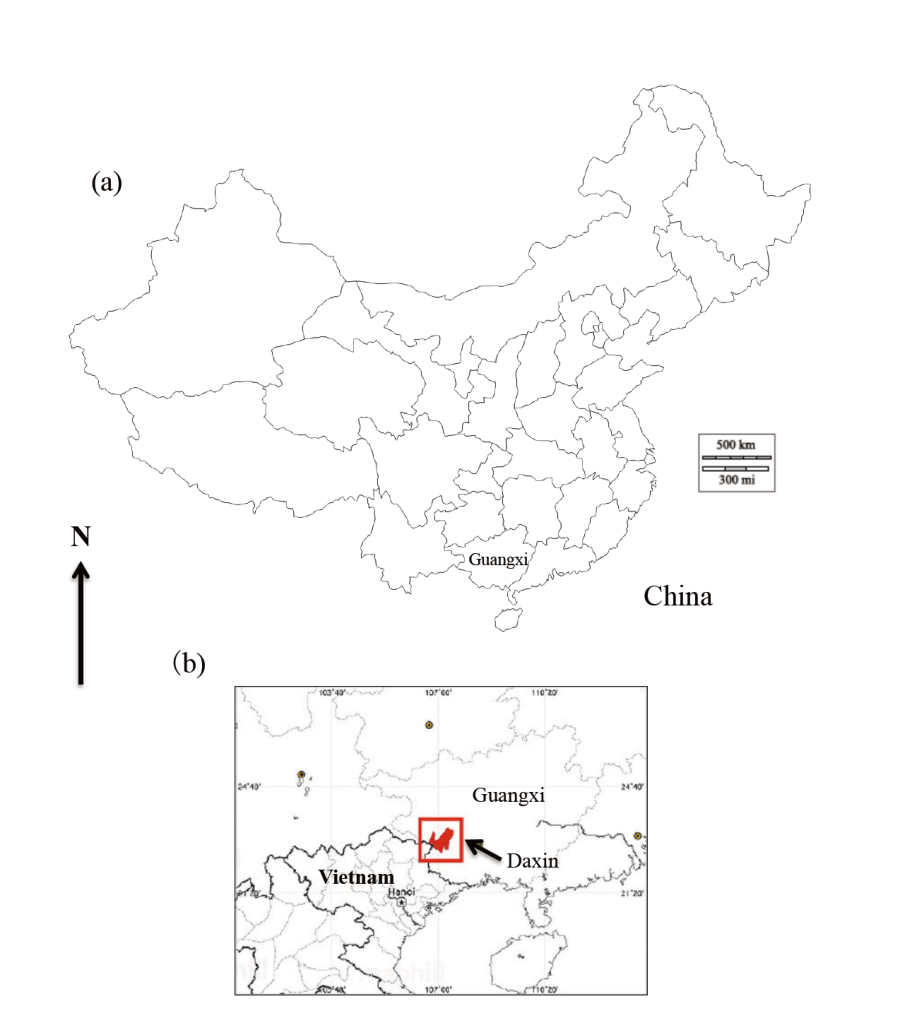
\includegraphics[scale=1]{Figures/Fig21.pdf}
  \caption[Locations of study sites]{Locations of study sites. (a) The Guangxi Zhuang Autonomous Region,
China, (b) the Daxin County (maps from www.maphill.com).}
\end{figure}

\begin{figure}
  \centering
    \label{fig:Fig22}
  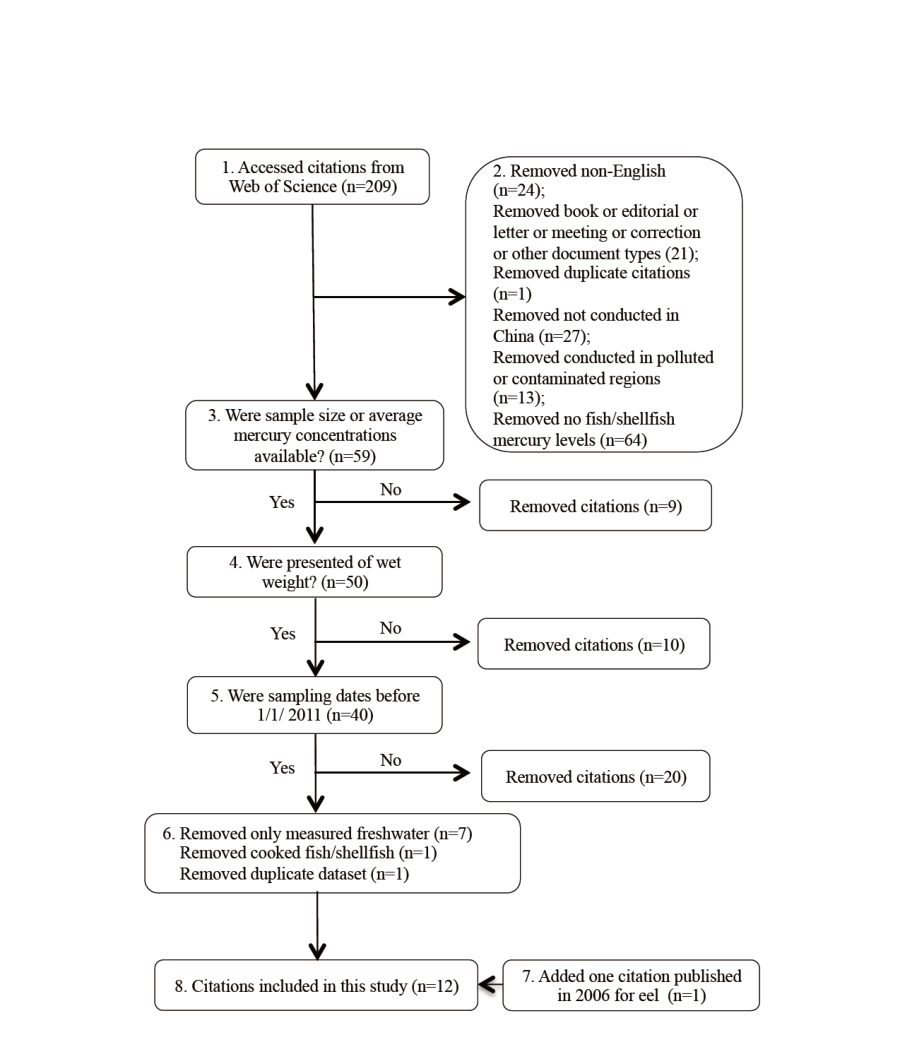
\includegraphics[scale=1]{Figures/Fig22.pdf}
  \caption[Flow chart of the literature search for the total mercury concentrations of
fish/shellfish]{Flow chart of the literature search for the total mercury concentrations of
fish/shellfish.}
\end{figure}

\begin{figure}
  \centering
    \label{fig:Fig23}
  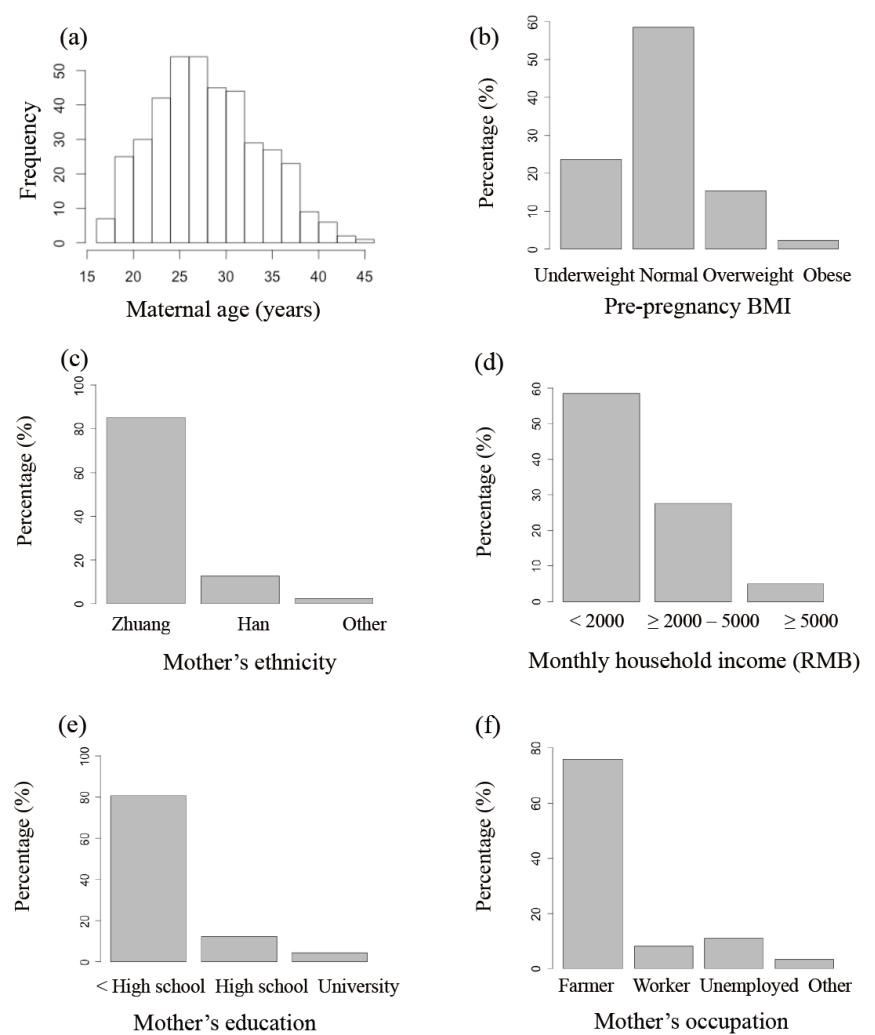
\includegraphics[scale=1]{Figures/Fig23.pdf}
  \caption[Distributions of (a) maternal age, (b) pre-pregnancy body mass index,
(c) mother's ethnicity, (d) monthly household income, (e) mother's education, and (d)
mother's occupation]{Distributions of (a) maternal age, (b) pre-pregnancy body mass index (BMI),
(c) mother's ethnicity, (d) monthly household income, (e) mother's education, and (d)
mother's occupation.}
\end{figure}

\begin{figure}
  \centering
    \label{fig:Fig24}
  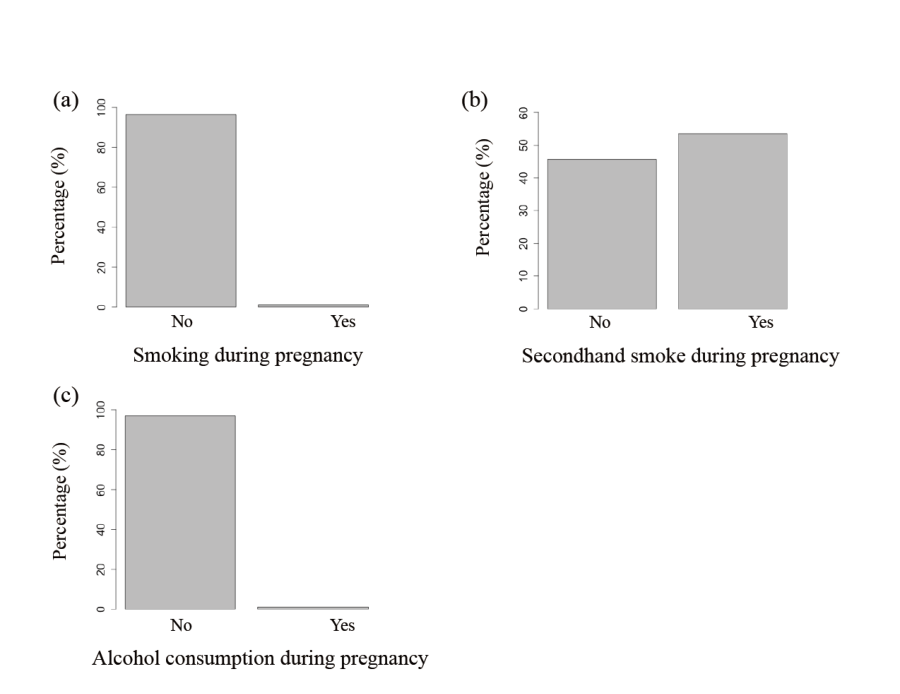
\includegraphics[scale=1]{Figures/Fig24.pdf}
  \caption[Distributions of (a) smoking during pregnancy, (b) secondhand smoke during
pregnancy, and (c) alcohol during pregnancy]{Distributions of (a) smoking during pregnancy, (b) secondhand smoke during pregnancy, and (c) alcohol during pregnancy.}
\end{figure}

\begin{figure}
  \centering
    \label{fig:Fig25}
  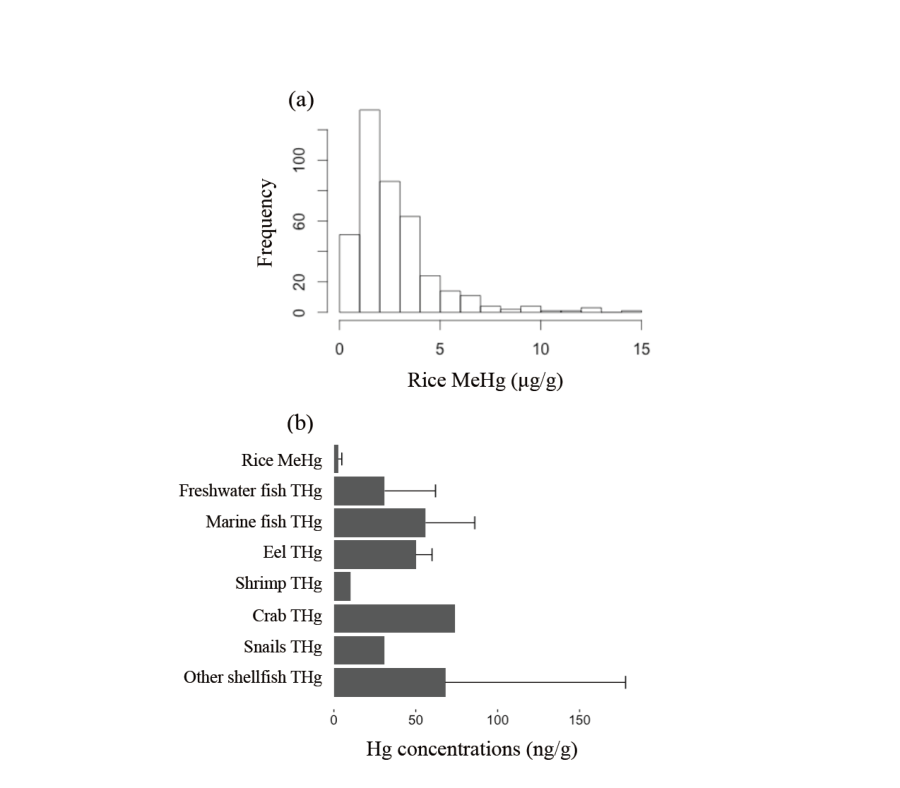
\includegraphics[scale=1]{Figures/Fig25.pdf}
  \caption[Distributions of rice and fish/shellfish mercury levels]{Distributions of rice and fish/shellfish mercury levels. (a) Histogram of the rice methylmercury (MeHg) concentrations, (b) bar chart of the rice MeHg concentrations and total mercury (THg) concentrations for each fish/shellfish variety. For marine fish and other shellfish, the average and SD were weighted based on sample size; for eel, the average and SD was provided by original study; for shrimp, crab, and
snails, the SD was not provided by original studies.}
\end{figure}

\begin{figure}
  \centering
    \label{fig:Fig26}
  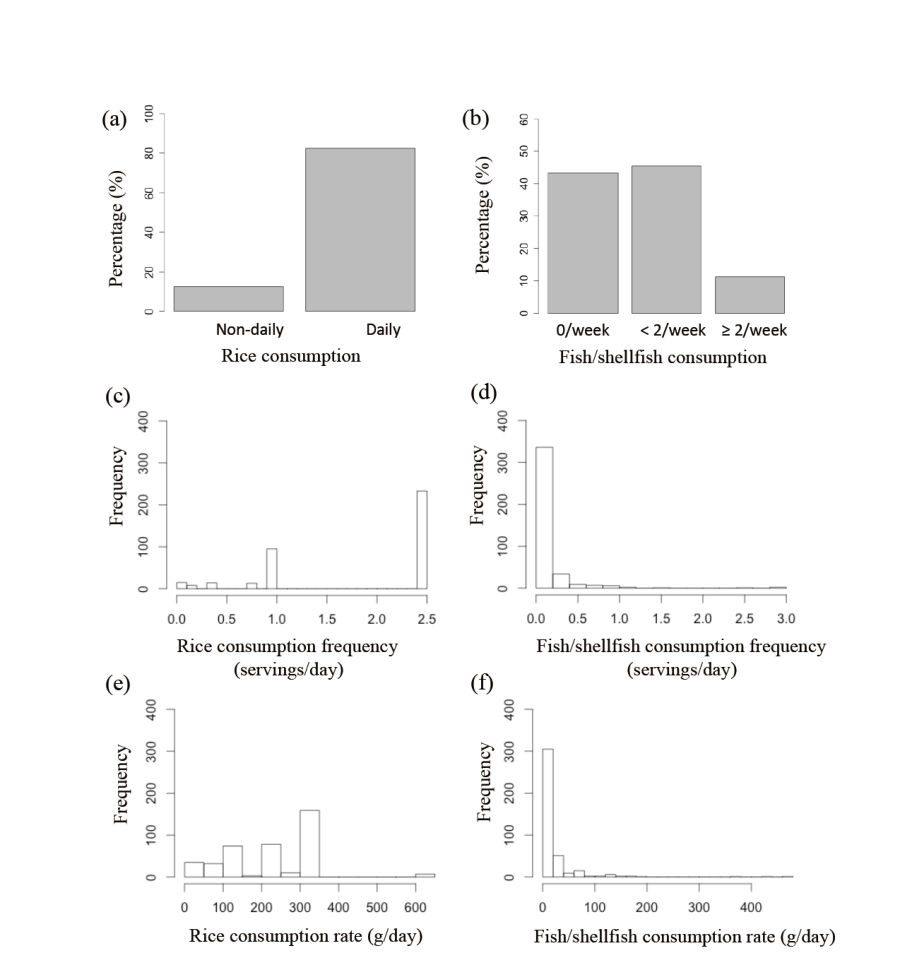
\includegraphics[scale=1]{Figures/Fig26.pdf}
  \caption[Distributions of rice consumption and fish/shellfish consumption]{Distributions of rice consumption and fish/shellfish consumption. (a) Rice consumption (non-daily vs. daily), (b) fish/shellfish consumption (rarely or never, < twice/week, ${\ge}$ twice/week), (c) rice consumption frequency (servings/day), (d) fish/shellfish consumption frequency (servings/day), (e) rice ingestion rate (g/day), and (f) fish/shellfish ingestion rate (g/day).}
\end{figure}

\begin{figure}
  \centering
    \label{fig:Fig27}
  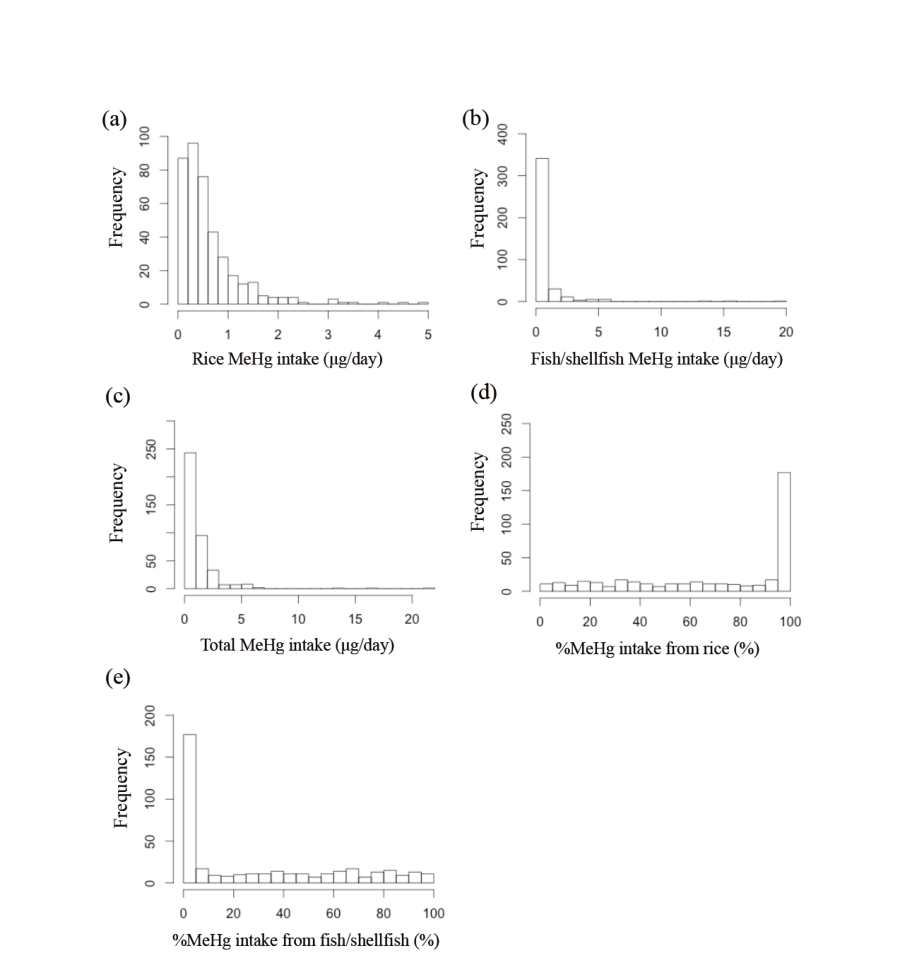
\includegraphics[scale=1]{Figures/Fig27.pdf}
  \caption[Distributions of rice and fish/shellfish methylmercury intake]{Distributions of rice and fish/shellfish methylmercury (MeHg) intake. (a) Rice MeHg intake, (b) fish/shellfish MeHg intake, (c) total MeHg intake through rice and fish/shellfish ingestion, (d) percentage of total MeHg intake from rice consumption, and (e) percentage of total MeHg intake from fish/shellfish consumption.}
\end{figure}

\begin{figure}
  \centering
    \label{fig:Fig28}
  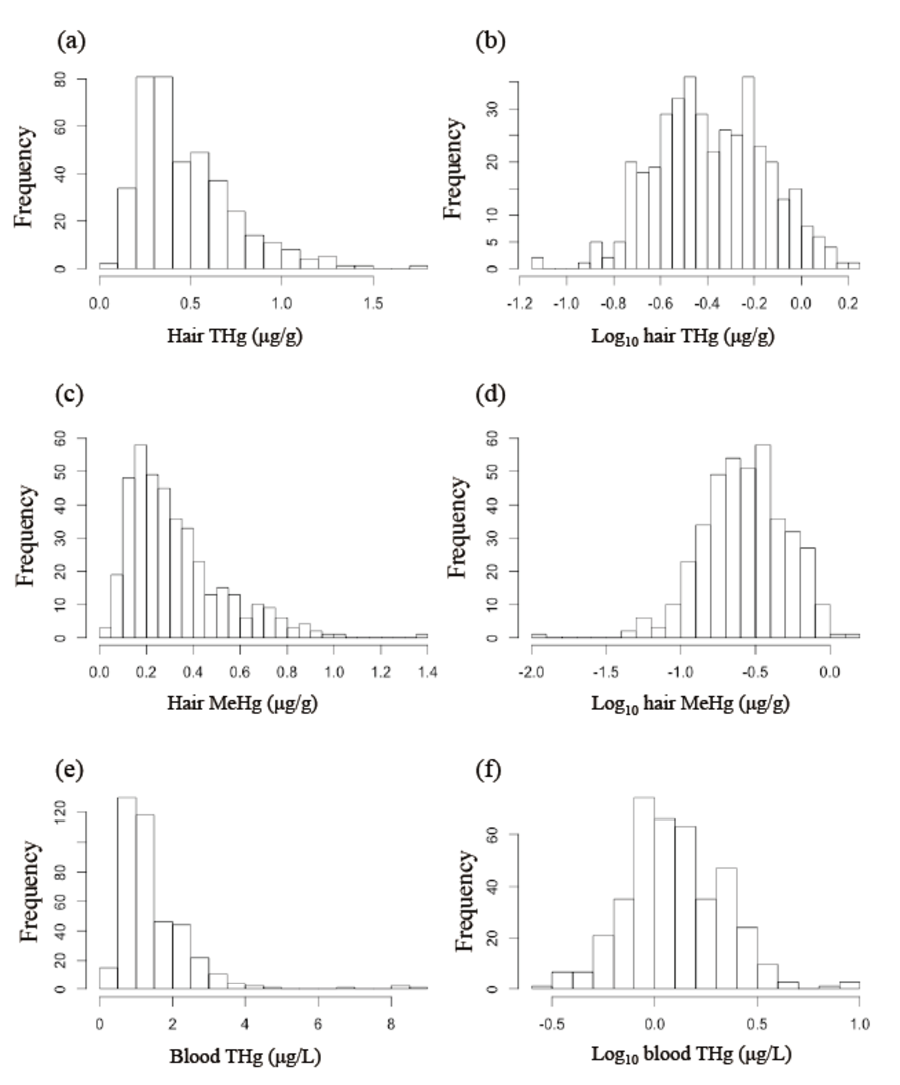
\includegraphics[scale=1]{Figures/Fig28.pdf}
  \caption[Histograms of (a) hair total mercury, (b) $\log_{10}$ hair total mercury, (c) hair methylmercury, (d) $\log_{10}$ hair methylmercury, (e) blood total mercury, and (f) $\log_{10}$ blood total mercury]{Histograms of (a) hair total mercury (THg), (b) $\log_{10}$ hair THg, (c) hair methylmercury (MeHg), (d) $\log_{10}$ hair MeHg, (e) blood THg, and (f) $\log_{10}$ blood THg}
\end{figure}

\begin{figure}
  \centering
    \label{fig:Fig29}
  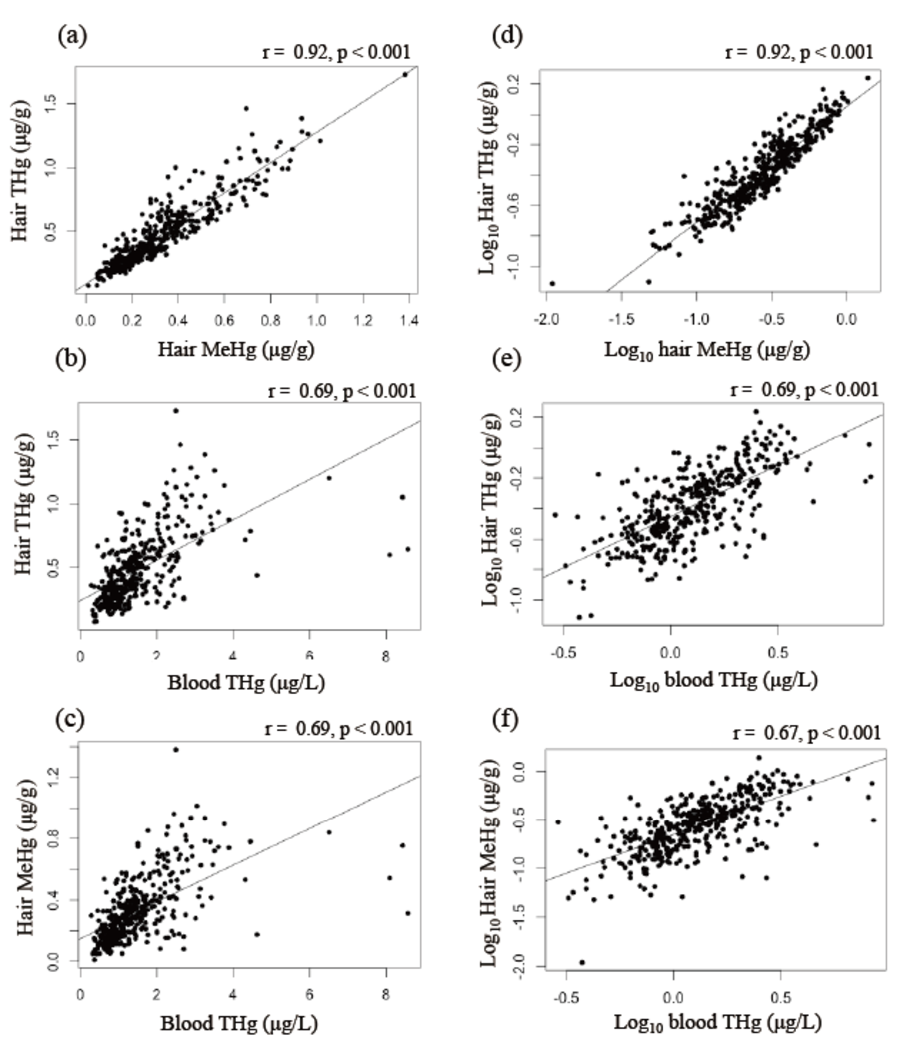
\includegraphics[scale=1]{Figures/Fig29.pdf}
  \caption[Bivariate analyses of hair total mercury, hair methylmercury, and blood total mercury.]{Bivariate analyses of hair total mercury (THg), hair methylmercury (MeHg), and blood THg. Spearman's correlation test for (a) hair MeHg vs. hair THg (r=0.92, p<0.001, n=398), (b) blood THg vs. hair THg (r=0.69, p<0.001, n=397), (c) blood THg vs. hair MeHg (r=0.69, p<0.001, n=397). Pearson's correlations test for (d) $\log_{10}$ hair MeHg vs. $\log_{10}$ hair MeHg (r=0.92, p<0.001, n=398), (e) $\log_{10}$ blood THg vs. $\log_{10}$ hair THg (r=0.69, p<0.001, n=397), (f) $\log_{10}$ blood THg vs. $\log_{10}$ hair MeHg (r=0.67, p<0.001, n=397).}
\end{figure}

\begin{figure}
  \centering
    \label{fig:Fig210}
  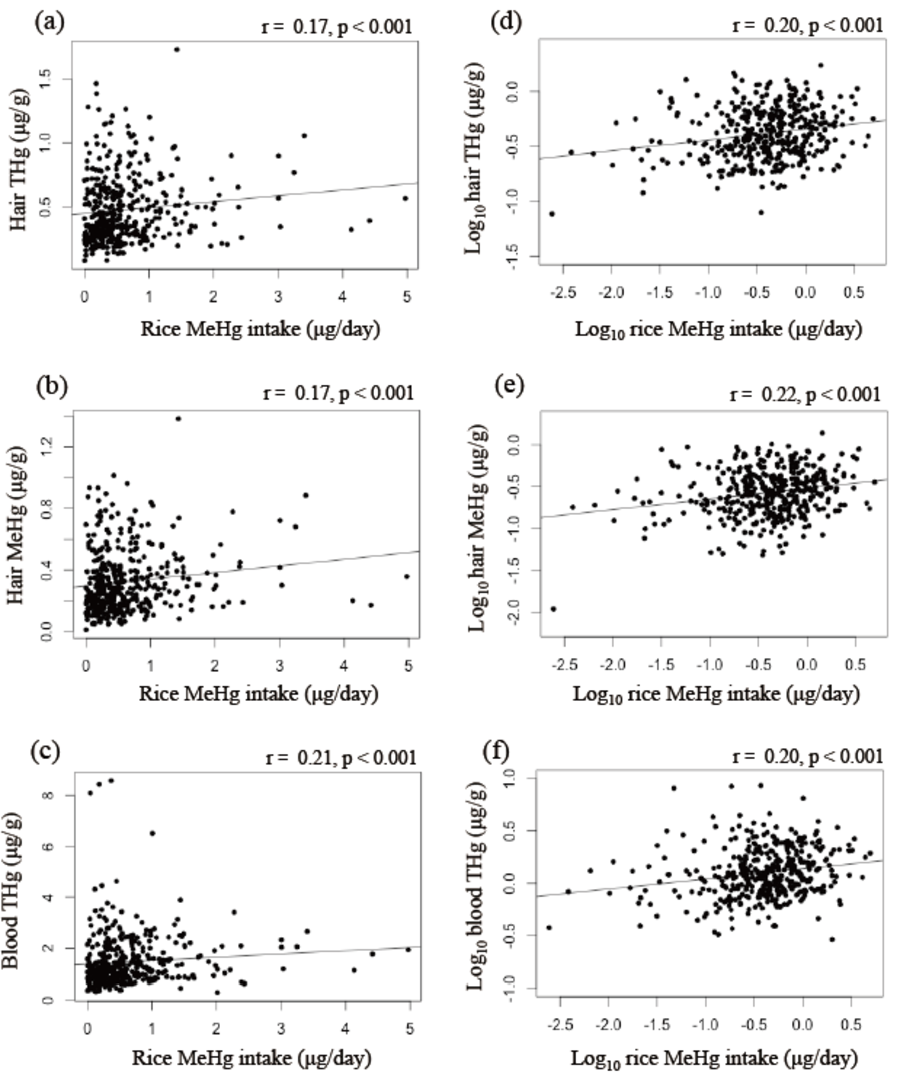
\includegraphics[scale=1]{Figures/Fig210.pdf}
  \caption[Bivariate analyses of rice methylmercury intake and mercury biomarkers]{Bivariate analyses of rice methylmercury (MeHg) intake and mercury biomarkers. Spearman's correlation test for (a) rice MeHg intake versus hair total mercury (THg) (r=0.17, p<0.001), (b) rice MeHg intake versus hair MeHg (r=0.17, p<0.001), (c) rice MeHg intake versus blood THg (r=0.21, p<0.001). Pearson's correlation test for (d) $\log_{10}$ rice MeHg intake versus $\log_{10}$ hair THg (r=0.20, p<0.001), (e) $\log_{10}$ rice MeHg intake versus $\log_{10}$ hair MeHg (r=0.22, p<0.001), and (f) $\log_{10}$ rice MeHg intake versus $\log_{10}$ blood THg (r=0.20, p<0.001) (n=397-398).}
\end{figure}

\begin{figure}
  \centering
    \label{fig:Fig211}
  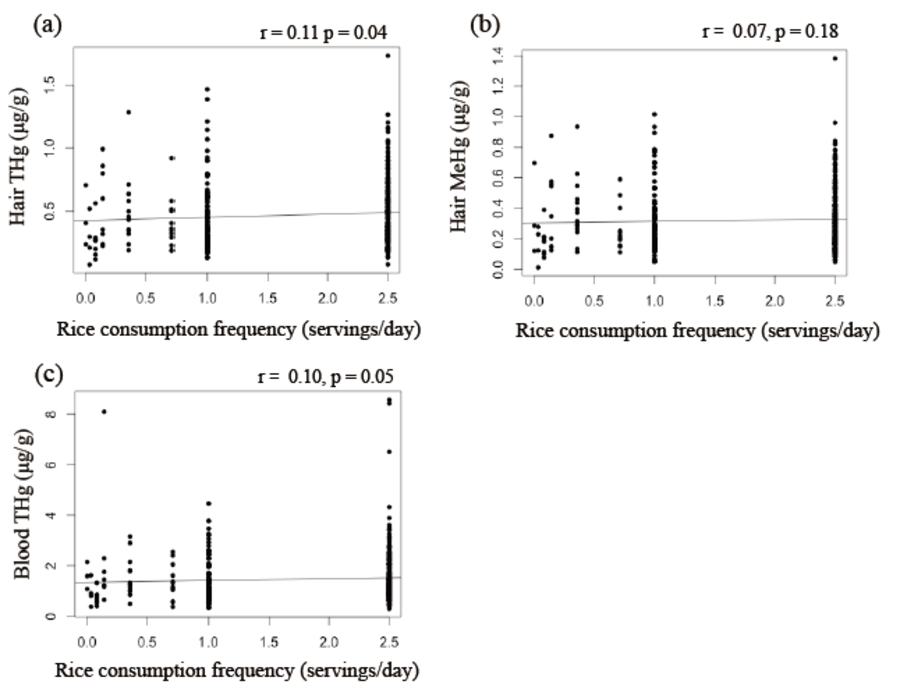
\includegraphics[scale=1]{Figures/Fig211.pdf}
  \caption[Bivariate analyses of rice consumption frequency and mercury biomarkers]{Bivariate analyses of rice consumption frequency and mercury biomarkers. (a) Rice consumption frequency versus hair total mercury (THg) (r=0.11, p=0.04), (b) rice consumption frequency versus hair methylmercury (MeHg) (r=0.07, p=0.18), (c) rice consumption frequency versus blood THg (r=0.10, p=0.05) (Spearman's correlation test for all, n=377-378).}
\end{figure}

\begin{figure}
  \centering
    \label{fig:Fig212}
  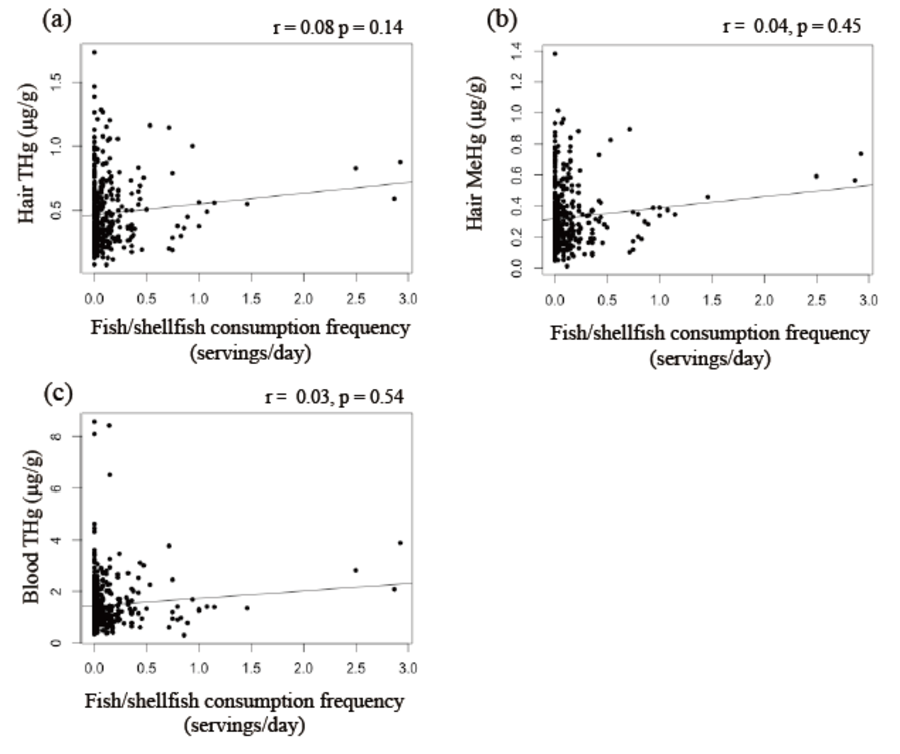
\includegraphics[scale=1]{Figures/Fig212.pdf}
  \caption[Bivariate analyses of fish/shellfish consumption frequency and mercury biomarkers]{Bivariate analyses of fish/shellfish consumption frequency and mercury biomarkers. (a) Fish/shellfish consumption frequency versus hair total mercury (THg) (r=0.08, p=0.14), (b) fish/shellfish consumption frequency versus hair methylmercury (MeHg) (r=0.04, p=0.45), (c) fish/shellfish consumption frequency versus blood THg (r=0.03, p=0.54) (Spearman's correlation test for all, n=397-398).}
\end{figure}

\begin{figure}
  \centering
    \label{fig:Fig213}
  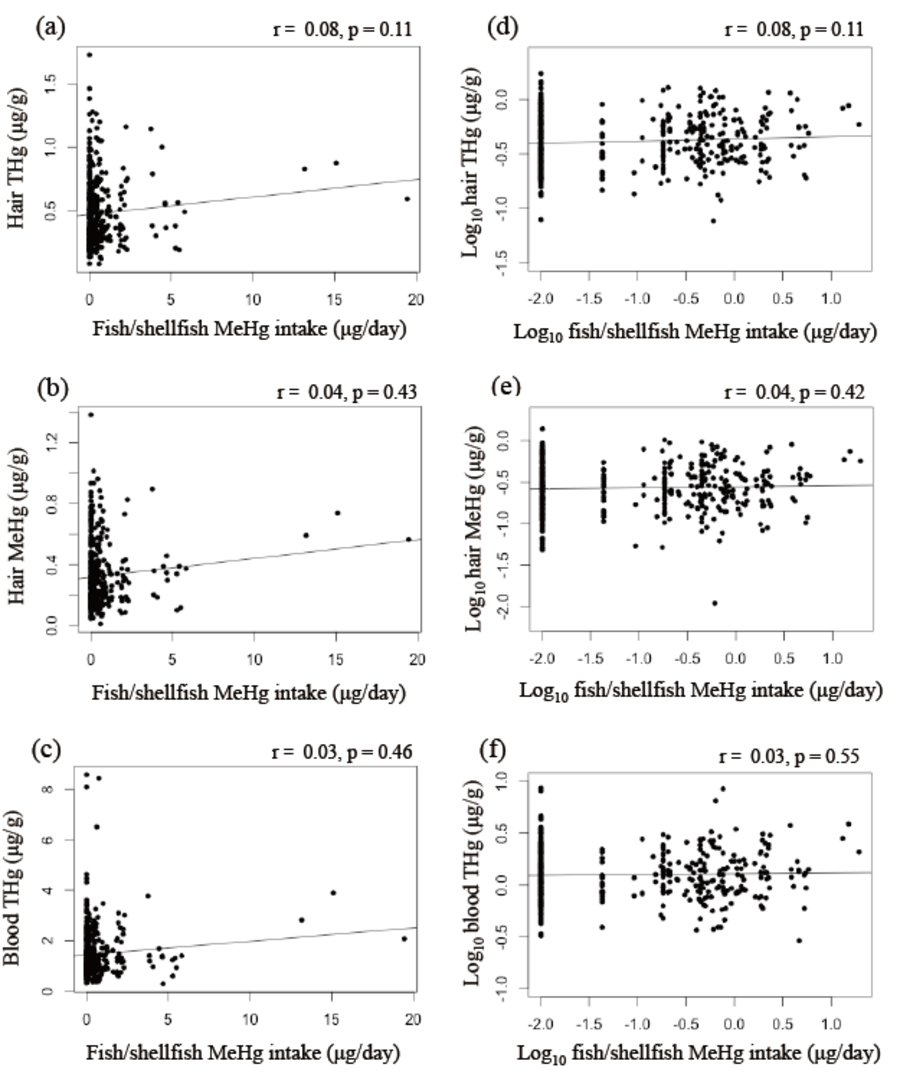
\includegraphics[scale=1]{Figures/Fig213.pdf}
  \caption[Bivariate analyses of fish/shellfish methylmercury intake and mercury biomarkers]{Bivariate analyses of fish/shellfish methylmercury (MeHg) intake and mercury biomarkers. Spearman's correlation test for (a) fish/shellfish MeHg intake versus hair total mercury (THg) (r=0.08, p=0.11), (b) fish/shellfish MeHg intake versus hair MeHg (r=0.04, p=0.45), (c) fish/shellfish MeHg intake versus blood THg (r=0.03, p=0.46). Pearson's correlation test for (d) $\log_{10}$ fish/shellfish MeHg intake versus $\log_{10}$ hair THg (r=0.08, p=0.11), (e) $\log_{10}$ fish/shellfish MeHg intake versus $\log_{10}$ hair MeHg (r=0.04, p=0.42), and (f) $\log_{10}$ fish/shellfish MeHg intake versus $\log_{10}$ blood THg (r=0.03, p=0.55) (n=397-398).}
\end{figure}

\begin{figure}
  \centering
    \label{fig:Fig214}
  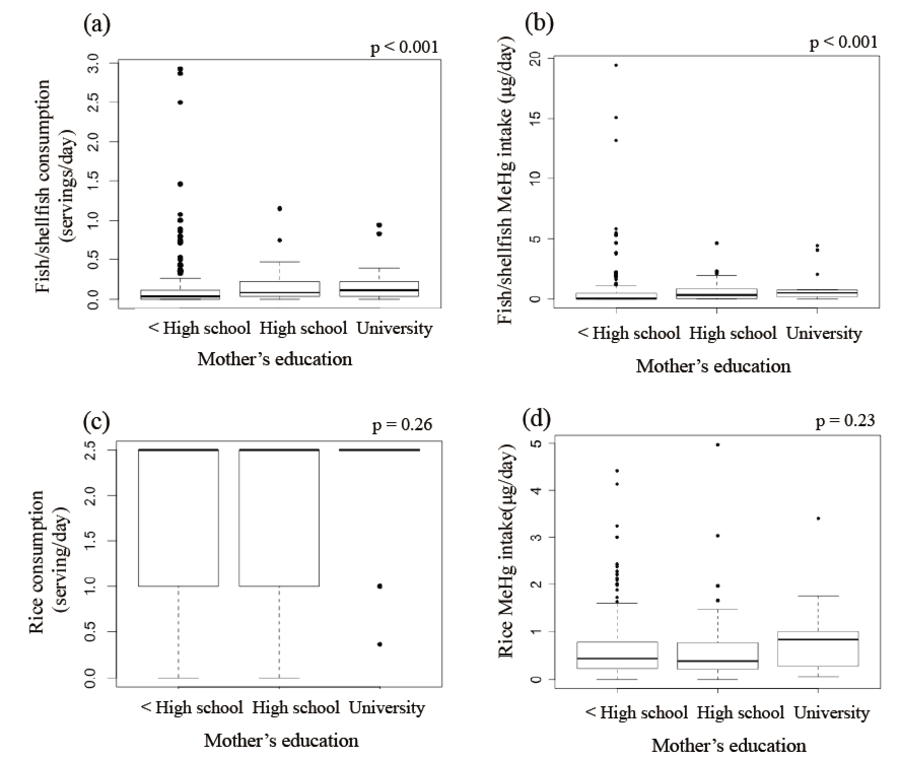
\includegraphics[scale=1]{Figures/Fig214.pdf}
  \caption[Bivariate analyses of mother's education versus fish/shellfish consumption frequency, fish/shellfish methylmercury intake, rice consumption frequency, and rice methylmercury intake]{Bivariate analyses of mother's education versus fish/shellfish consumption frequency, fish/shellfish methylmercury (MeHg) intake, rice consumption frequency, and rice MeHg intake. (a) Education versus fish/shellfish consumption frequency (p<0.001), (b) education versus fish/shellfish MeHg intake (p<0.001)) (c) education versus rice consumption frequency (p=0.26), (d) education versus rice MeHg intake (p=0.23) (Kruskal-Wallis test for all, n=386-388).}
\end{figure}

\begin{figure}
  \centering
    \label{fig:Fig215}
  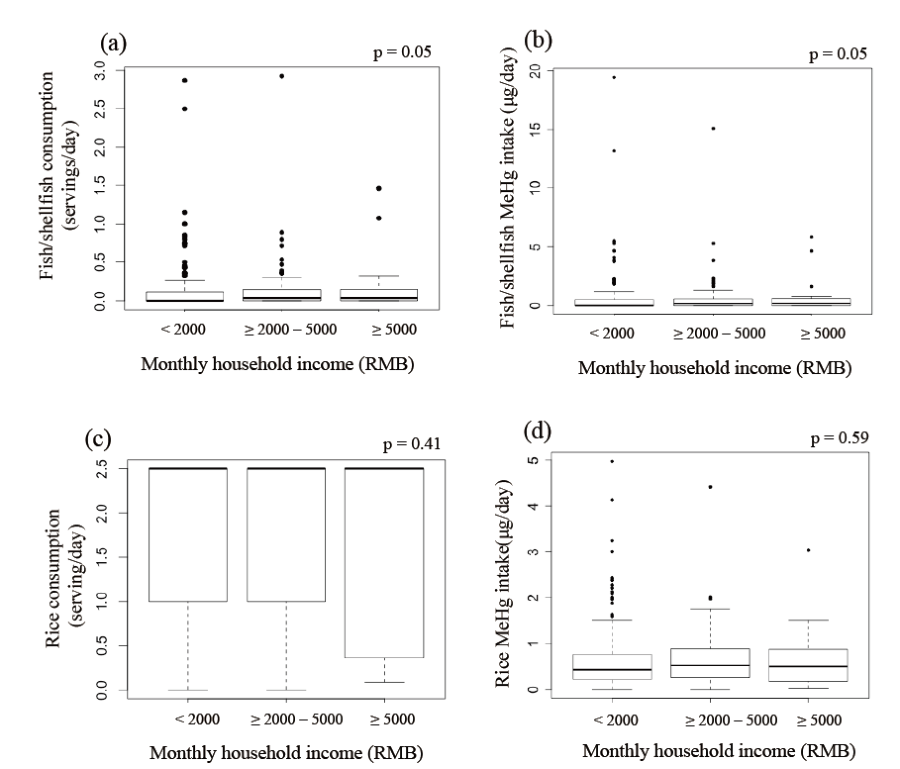
\includegraphics[scale=1]{Figures/Fig215.pdf}
  \caption[Bivariate analyses of monthly household income versus fish/shellfish consumption frequency, fish/shellfish methylmercury intake, rice consumption frequency, and rice methylmercury intake]{Bivariate analyses of monthly household income versus fish/shellfish consumption frequency, fish/shellfish methylmercury (MeHg) intake, rice consumption frequency, and rice MeHg intake. (a) Income versus fish/shellfish consumption frequency (p=0.05), (b) income versus fish/shellfish MeHg intake (p=0.05), (c) income versus rice consumption frequency (p=0.41), (d) income versus rice MeHg intake (p=0.59) (Kruskal-Wallis test for all, n=361-363).}
\end{figure}

\begin{figure}
  \centering
    \label{fig:Fig216}
  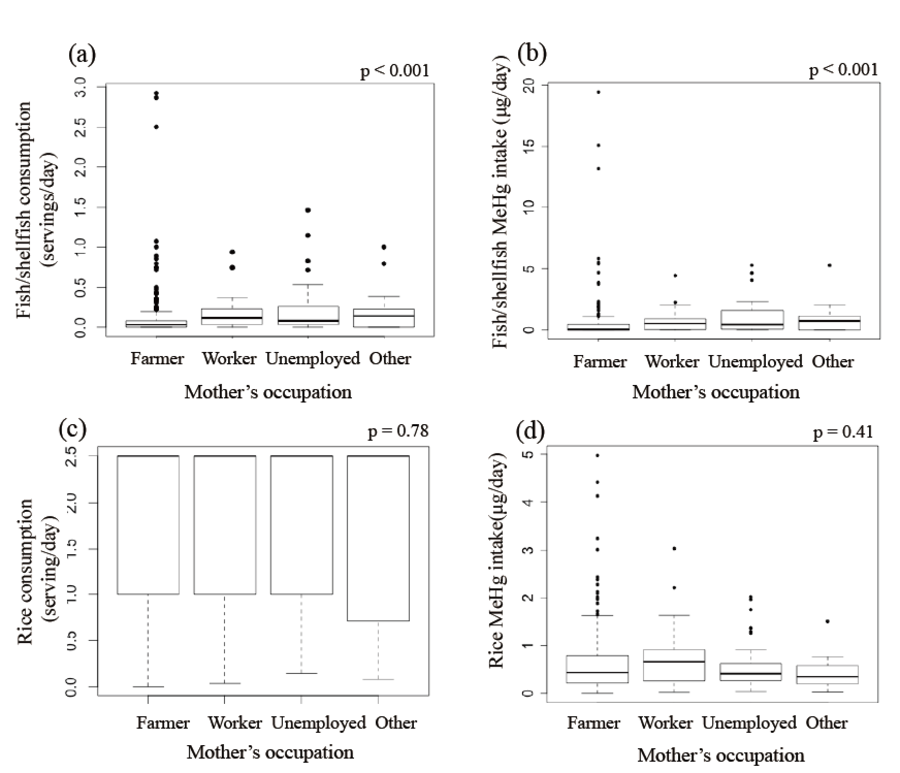
\includegraphics[scale=1]{Figures/Fig216.pdf}
  \caption[Bivariate analyses of mother's occupation versus income versus fish/shellfish consumption frequency, fish/shellfish methylmercury intake, rice consumption frequency, and rice methylmercury intake]{Bivariate analyses of mother's occupation versus income versus fish/shellfish consumption frequency, fish/shellfish methylmercury (MeHg) intake, rice consumption frequency, and rice MeHg intake. (a) Occupation versus fish/shellfish consumption frequency (p<0.001), (b) occupation versus fish/shellfish MeHg intake (p<0.001), (c) occupation versus rice consumption frequency (p=0.78), (d) occupation versus rice MeHg
intake (p=0.41) (Kruskal-Wallis test for all, n=389-391).}
\end{figure}


\begin{figure}
  \centering
    \label{fig:Fig217}
  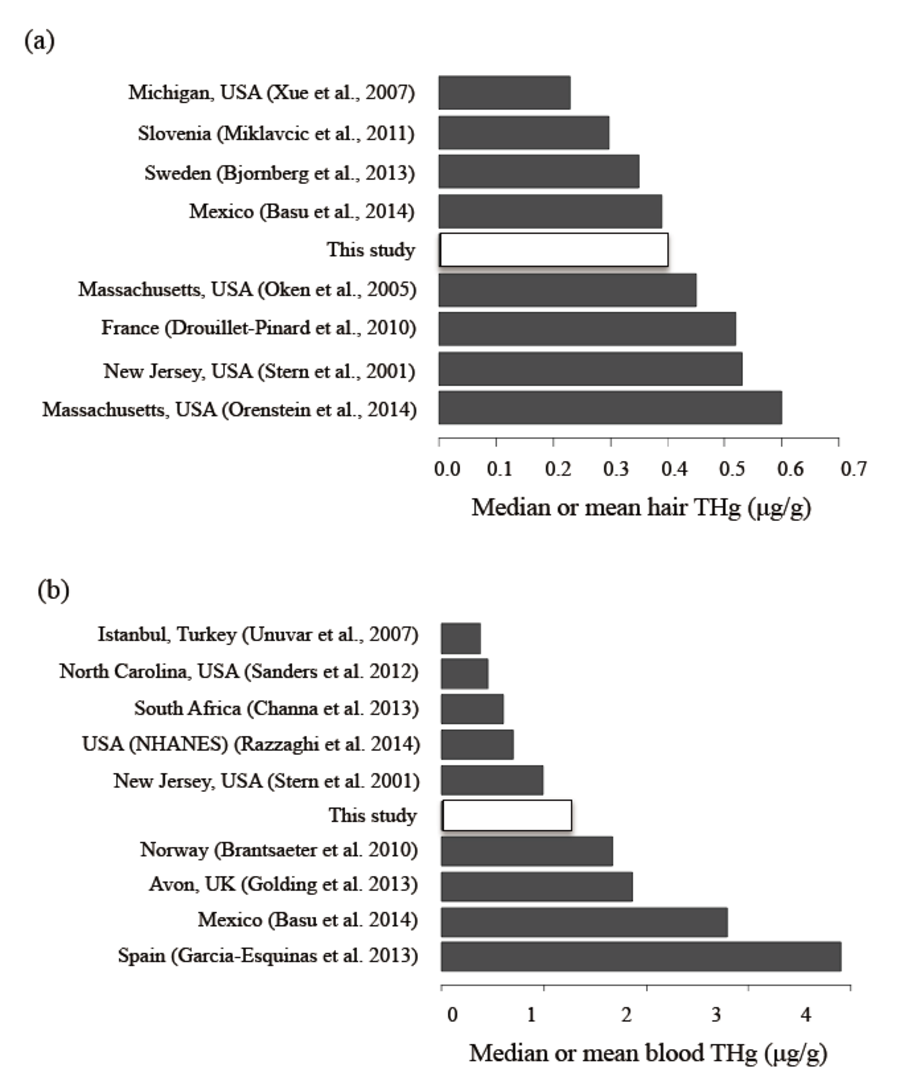
\includegraphics[scale=1]{Figures/Fig217.pdf}
  \caption[Summary of median or mean total mercury concentrations in (a) maternal hair and (b) maternal blood, from studies among pregnant women with low-level mercury exposure]{Summary of median or mean total mercury (THg) concentrations in (a) maternal hair and (b) maternal blood, from studies among pregnant women with low-level mercury exposure (see Table 2.7 for more detail).}
\end{figure}

